\documentclass[aspectratio=43]{beamer}
\mode<beamer>

% [A] Theme Stuff
\usetheme{CambridgeUS}
\usecolortheme{beaver}
\definecolor{miamired}{RGB}{200,16,46}
\definecolor{darkgreen}{rgb}{0.09, 0.45, 0.27}
%\setbeamertemplate{footline}[frame number]
\setbeamercolor{title}{fg=miamired}
\setbeamercolor{block title}{bg=gray!35,fg=black}
\setbeamercolor{block body}{bg=gray!0,fg=black}
\setbeamercolor{frametitle}{fg=miamired}
\usefonttheme[]{serif}
\setbeamertemplate{items}[ball]
\setbeamercolor{alerted text}{fg=miamired,bg=}
\setbeamercolor*{item}{fg=miamired}
\setbeamercolor{section number projected}{bg=miamired}
\setbeamercolor{colorbox}{bg=miamired, fg=white}
\setbeamercolor{section in head/foot}{bg=miamired}
\setbeamercolor{author in head/foot}{bg=miamired}
\setbeamercolor{bibliography entry author}{fg=miamired}
\setbeamercolor{bibliography entry title}{fg=black} 
\setbeamercolor{bibliography entry location}{fg=miamired} 
\setbeamercolor{bibliography entry note}{fg=black!85}
\setbeamertemplate{bibliography item}[text]
%\setbeamertemplate{bibliography item}[article] % To have an article instead of the number
% https://tex.stackexchange.com/questions/183052/what-are-all-the-possible-first-arguments-to-setbeamerfont/183053#183053
\setbeamerfont{alerted text}{series=\bfseries}
\setbeamerfont{block title}{series=\bfseries}
\setbeamerfont{block body}{series=\bfseries}
\setbeamerfont{itemize item}{series=\bfseries}
\setbeamerfont*{itemize/enumerate subbody}{parent=itemize/enumerate body}
\setbeamerfont*{itemize/enumerate subsubbody}{parent=itemize/enumerate body}
\setbeamerfont{section in toc}{series=\bfseries}
\setbeamerfont{frametitle}{series=\bfseries}
\setbeamerfont{footline}{series=\tiny}
\setbeamerfont{headlineline}{series=\tiny}
\setbeamerfont{section in head/foot}{series=\tiny}
\setbeamerfont{subsection in head/foot}{series=\tiny}
\setbeamerfont{subsubsection in head/foot}{series=\tiny}
\setbeamerfont{page number in head/foot}{series=\tiny}
\setbeamerfont{date}{series=\scriptsize}
\setbeamerfont{date in head/foot}{series=\tiny}
\setbeamercolor*{block title example}{fg=miamired,
	bg=miamired!10}
\setbeamercolor*{block body example}{fg= black}

\setbeamerfont{bibliography item}{size=\footnotesize}
\setbeamerfont{bibliography entry author}{size=\footnotesize}
\setbeamerfont{bibliography entry title}{size=\footnotesize}
\setbeamerfont{bibliography entry location}{size=\footnotesize}
\setbeamerfont{bibliography entry note}{size=\footnotesize}

% [B] Needed Packages
\usepackage[export]{adjustbox}
\usepackage{amsfonts}
\usepackage{amsmath}
\usepackage{amssymb}
\usepackage{animate}
\usepackage{array}
\newcolumntype{m}[1]{>{\arraybackslash\hspace{0pt}}p{#1}}
\usepackage[justification=centering]{caption}
\usepackage{colortbl}
\usepackage{etoolbox}
\usepackage{fancybox}
\usepackage{framed}
\usepackage{graphics}
\usepackage{graphicx}
\usepackage{hyperref} 
\usepackage[utf8]{inputenc}
\usepackage{makecell}
\usepackage{mathtools}
\usepackage{marvosym}
\usepackage[framemethod=default]{mdframed}
\usepackage{media9}
%\addmediapath{./Figures/}
\usepackage{multicol}
%\usepackage{multimedia}
\usepackage{multirow}
\usepackage{pgfplots} %for tikzpictures
\usepackage{sidecap}
\usepackage{smartdiagram}
\usepackage{soul}
\usepackage{subfigure}
\usepackage{tikz}
\usetikzlibrary{shapes.geometric, arrows}
\usepackage{times}
\usepackage{url}
	\urlstyle{same}
\usepackage{wasysym} % for smiley faces
\usepackage{wrapfig}








% [C] New Commands and Default Pathes
\newcommand{\norm}[1]{\left\lVert#1\right\rVert}
\graphicspath{ {Figures/} }
\setbeamertemplate{frametitle continuation}{[\insertcontinuationcount]}
\setbeamercovered{still covered={\opaqueness<1->{5}},again covered={\opaqueness<1->{60}}}
% begining of the new definition
\makeatletter
\newcommand*\fix@beamer@close{%
	\ifnum\beamer@trivlistdepth>0
	\beamer@closeitem
	\fi
}
\newcommand*\fix@beamer@open{%
	\ifnum\beamer@trivlistdepth>0
	\gdef\beamer@closeitem{}%
	\fi
}
\BeforeBeginEnvironment{itemize}{\fix@beamer@close}
\AfterEndEnvironment{itemize}{\fix@beamer@open}
\makeatother
% end of the new definition

% For Boxes
\newmdenv[skipabove=7pt,
skipbelow=7pt,
rightline=false,
leftline=true,
topline=false,
bottomline=false,
backgroundcolor= miamired!10,
linecolor= miamired,
innerleftmargin=5pt,
innerrightmargin=5pt,
innertopmargin=5pt,
innerbottommargin=5pt,
leftmargin=0cm,
rightmargin=0cm,
linewidth=4pt]{eBox}

\newmdenv[skipabove=7pt,
skipbelow=7pt,
rightline=false,
leftline=true,
topline=false,
bottomline=false,
linecolor=miamired,
innerleftmargin=5pt,
innerrightmargin=5pt,
innertopmargin=0pt,
leftmargin=0cm,
rightmargin=0cm,
linewidth=4pt,
innerbottommargin=0pt]{dBox}

\newtheorem{exampleT}{Example}[section]
\newenvironment{ExamplesT}{\begin{exampleT}}{\hfill{\tiny\ensuremath{\blacksquare}}\end{exampleT}}


\newenvironment{conditions}
{\par\vspace{\abovedisplayskip}\noindent\begin{tabular}{>{$}l<{$} @{${}={}$} l}}
	{\end{tabular}\par\vspace{\belowdisplayskip}}
%%%%%%%%%%%%%%%%%%%%%%%%%%%%%%%%%%%%%%%%%%%%%%%%%%%%%%%%%%%%%%


\AtBeginSection[]
{
	\begin{frame}{Outline}
	\tableofcontents[currentsection, %subsectionstyle=show/shaded/hide,
	subsectionstyle=hide,
	subsubsectionstyle=hide]
\end{frame}
}

%\AtBeginSubsection[]
%{
%\begin{frame}{Outline}
%\tableofcontents[currentsection, %subsectionstyle=show/shaded/hide, %subsubsectionstyle=hide]
%\end{frame}
%}
\usepackage{svg}
\svgsetup{inkscapelatex=false}

%____________________ Title, Author, Affliation & Date____________________
\title[SPC \& Human Performance Modeling]{A Statistical (Process Monitoring) Perspective on Human Performance Modeling in the Age of Cyber-Physical Systems}
%\subtitle[Perspective and Guidelines]{Applications in Manufacturing, Transportation and Health Management}

\author[Fadel M. Megahed]{Fadel M. Megahed\inst{1}, L. Allison Jones-Farmer\inst{1}, Miao Cai\inst{2}, Steven E. Rigdon\inst{2} and Manar Mohamed \inst{1}}
\institute[Miami University]{\inst{1} Miami University, OH, USA \and \inst{2} Saint Louis University, MO, USA}


\date[ISQC 2019]{August 14\textsuperscript{th}, 2019}
%%%%%%%%%%%%%%%%%%%%%%%%%%%%%%%%%%%%%%%%%%%%%%%%%%%%%%%%%%%%%%%%%%%%%%%%%%

\begin{document}

% Frame 1
\maketitle


\section{Preface}
% Frame 3
\begin{frame}{\textbf{My Research Portfolio's Evolution}}
    \centering
    \only<1>{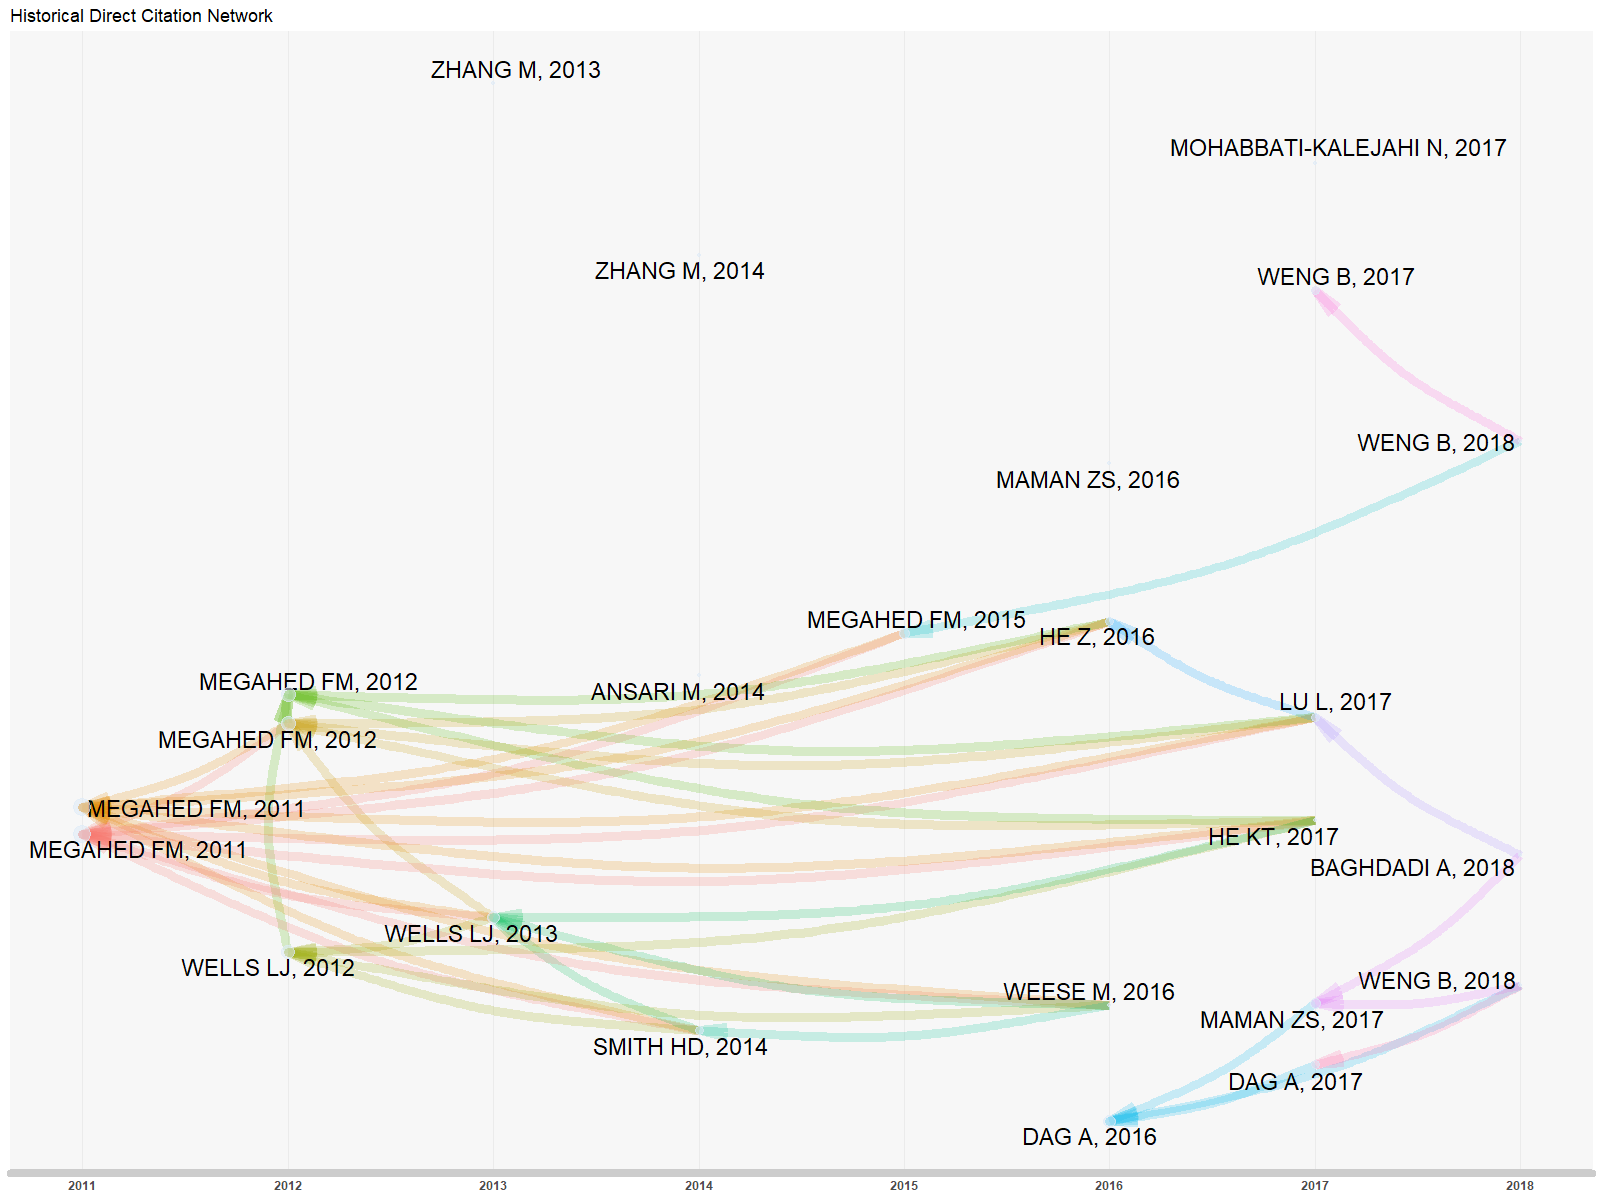
\includegraphics[height=0.8\textheight,
    width=\textwidth, keepaspectratio, frame]{Figures/historymegahed.png}}
    
    \only<2>{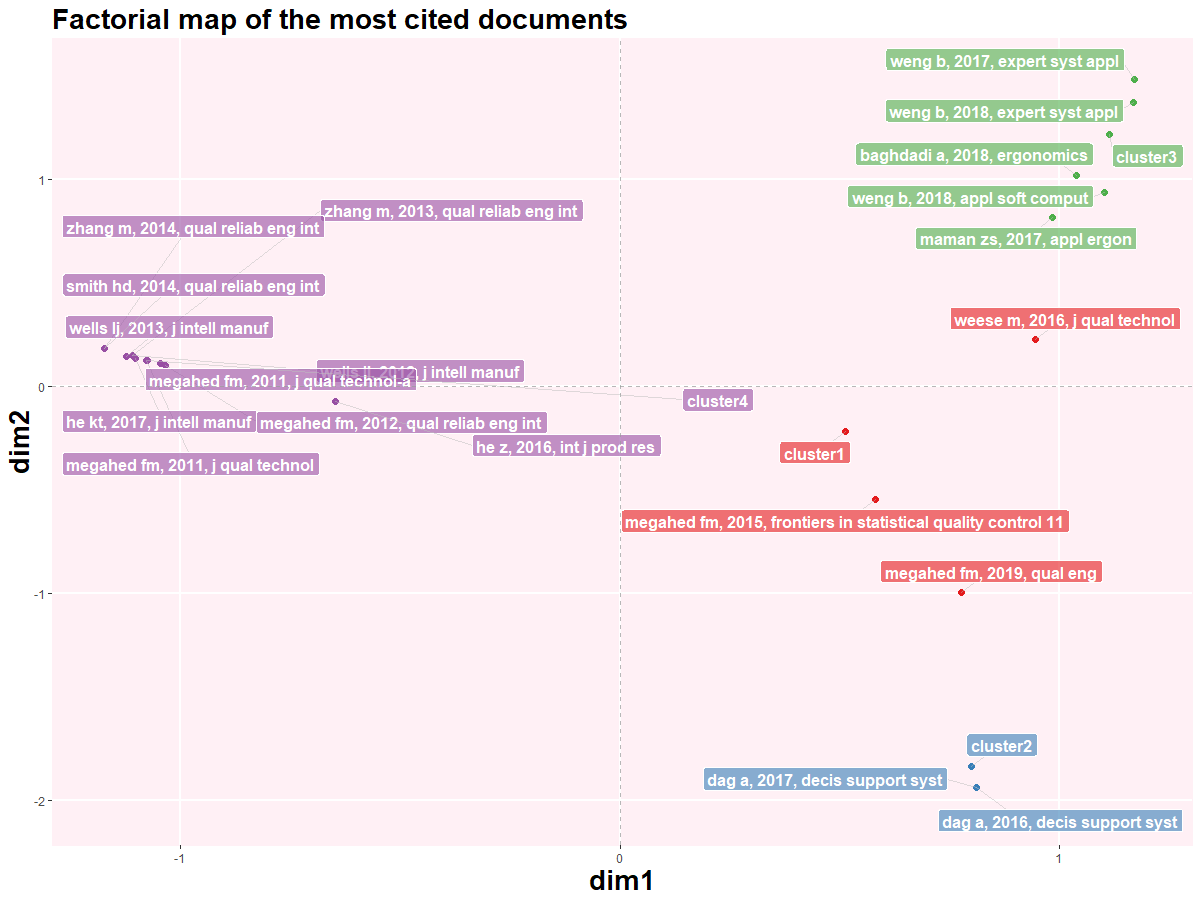
\includegraphics[height=0.8\textheight,
    width=\textwidth, keepaspectratio, frame]{Figures/papersmegahed.png}}
    
    \only<3>{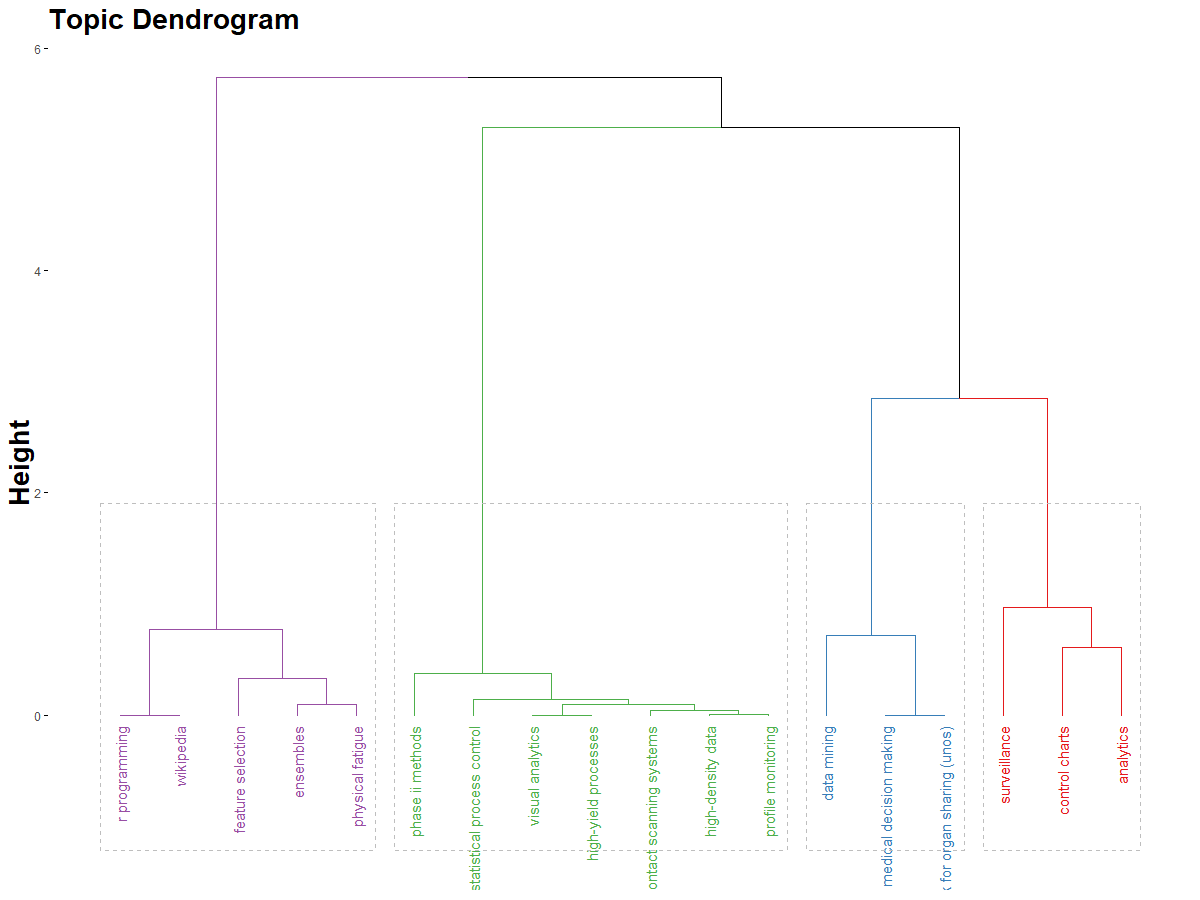
\includegraphics[height=0.8\textheight,
    width=\textwidth, keepaspectratio, frame]{Figures/dendomegahed.png}}
\end{frame}

\section{The Era of Cyber-Physical Systems (CPS)}

\subsection{Perspectives from Industry and Governing Research Bodies}

% Frame 5
\begin{frame}{\textbf{Gartner's Hype Cycle for Emerging Technologies}}
    \centering
    \href{https://www.gartner.com/smarterwithgartner/5-trends-emerge-in-gartner-hype-cycle-for-emerging-technologies-2018/}{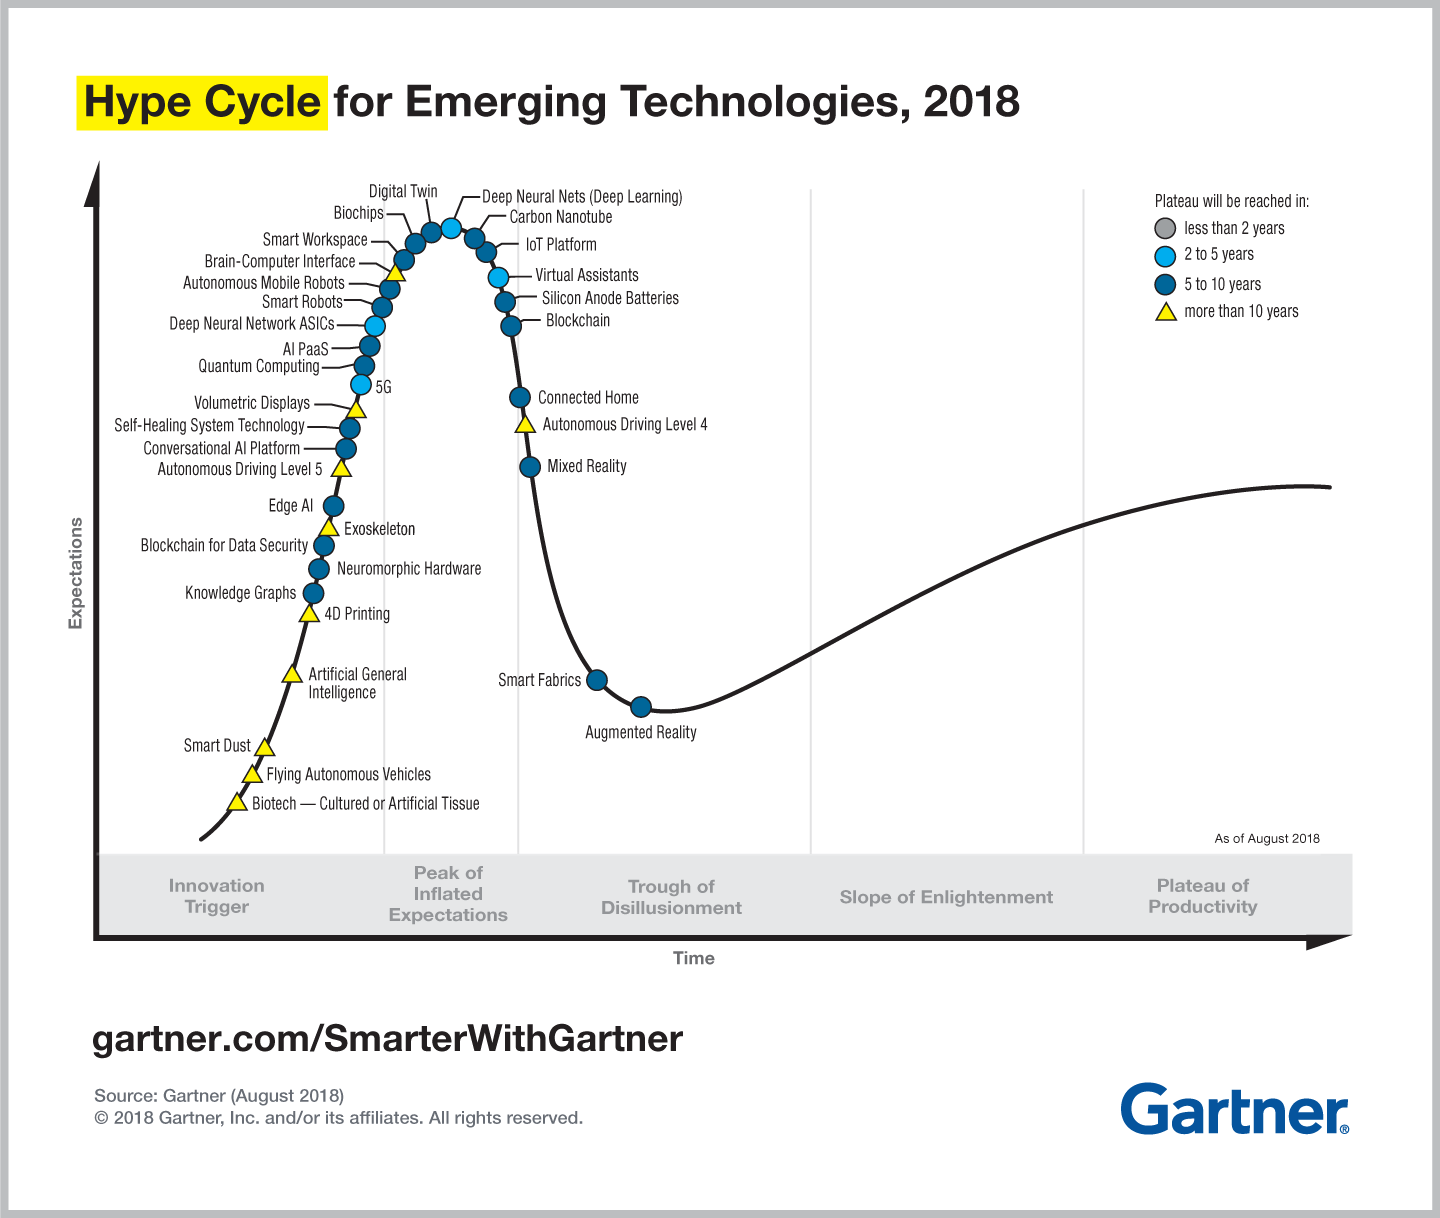
\includegraphics[width=\textwidth, height=0.8\textheight, frame]{Figures/2018_Hype_Cycle.png}}
\end{frame}

% Frame 6
\begin{frame}{\textbf{NSF's Alignment with the Gartner's Perspective}}
            ``Cyber-physical systems (CPS) are engineered systems that are built from, and depend upon, the seamless integration of computation and physical components. Advances in CPS will enable capability, adaptability, scalability, resiliency, safety, security, and usability that will expand the horizons of these critical systems. CPS technologies are transforming the way people interact with engineered systems, just as the Internet has transformed the way people interact with information. New, smart CPS drive innovation and competition in a range of application domains including agriculture, aeronautics, building design, civil infrastructure, energy, environmental quality, healthcare and personalized medicine, manufacturing, and transportation. Moreover, the \textcolor{miamired}{integration of artificial intelligence with CPS creates new research opportunities with major societal implications.}" \cite{nsf2019cps}
\end{frame}

% Frame 7
\begin{frame}{\textbf{Expected Value for CPS Applications}}
    \centering 
    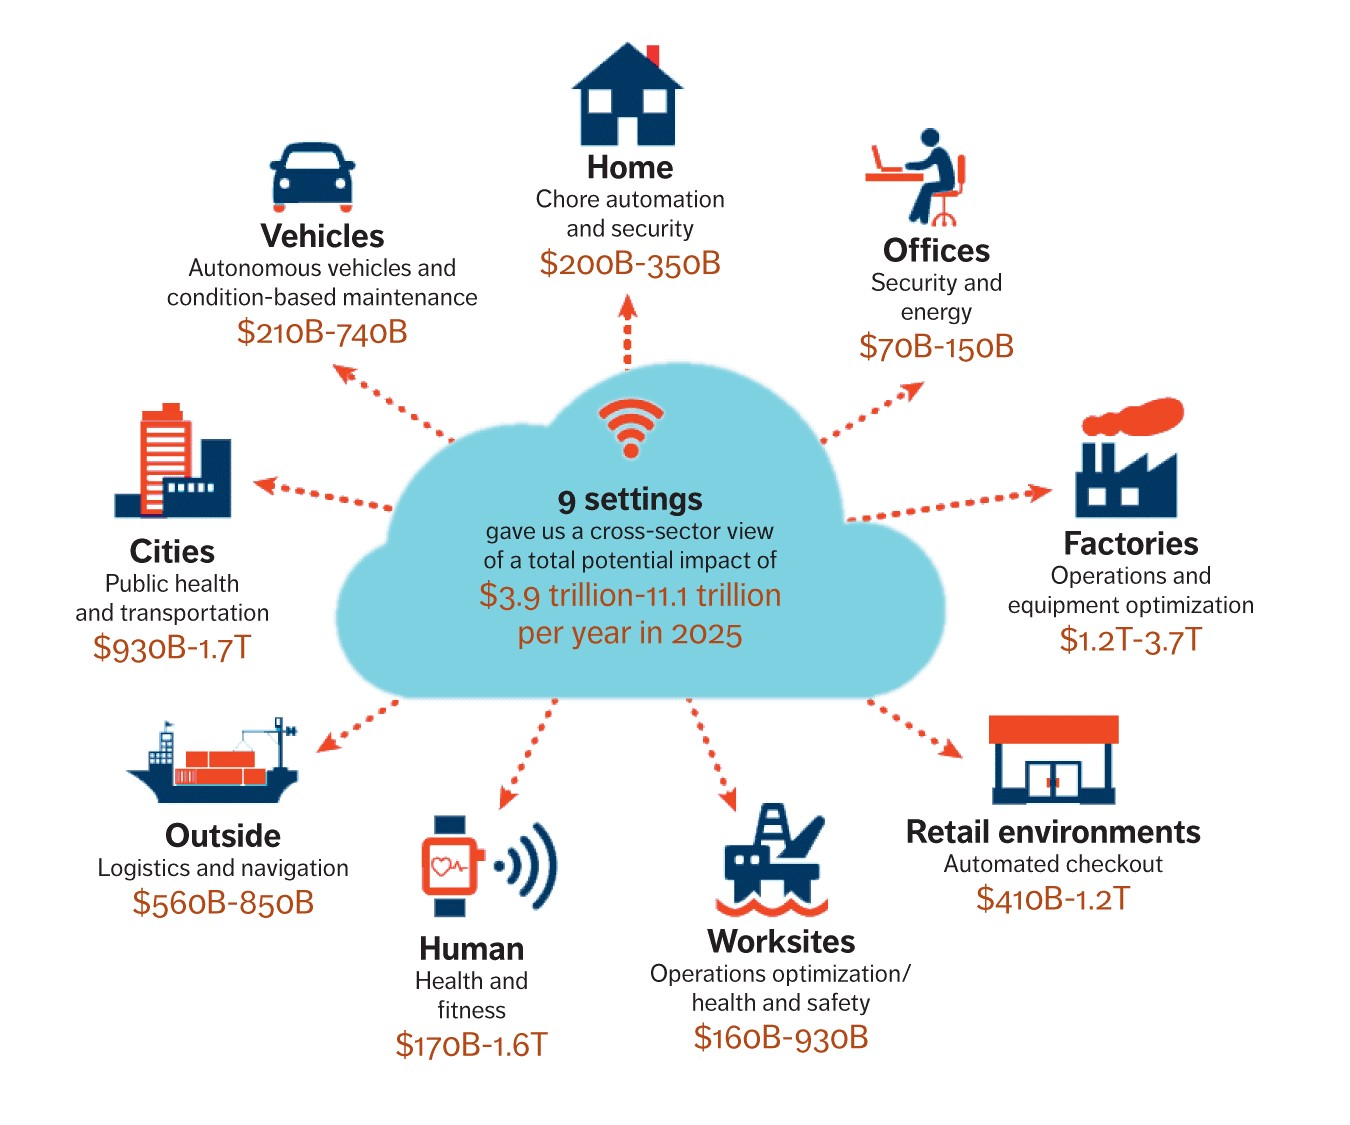
\includegraphics[width=\textwidth, height= 0.77\textheight, keepaspectratio, frame]{Figures/McKinsey-Global-Institute_IoT.jpg} 
    
    \tiny{\textbf{Source:} McKinsey\&Company. The McKinsey Global Institute \cite{mckinsey2015}.}
 
\end{frame}

\subsection{A Human-Centered Look on Cyber-Physical Systems}
% Frame 8
\begin{frame}{\textbf{Humans: A Cornerstone of CPS/IoT Applications}}
    \begin{itemize}
        \item<1-5> \textbf{From the McKinsey report \cite{mckinsey2015}, one can argue that data pertaining to human/workers is important to the following five applications:}
        \begin{itemize}[<+>]
            \item \textbf{Factories [Market size: \$1.2T-3.7T]}
            \item \textbf{Human health and fitness [Market size: \$170B-1.6T]}
            \item \textbf{Worksites [Market size: \$160B-930B]}
            \item \textbf{Logistics and Navigation [Market size: \$560B-850B]}
            \item \textbf{Offices [Market size: \$70B-150B]}
        \end{itemize}
        \item<6> \textbf{At a minimum, the market size for these five applications is estimated to be \$2.16T in 2025.}
    \end{itemize}
    
    \only<7>{
        \begin{eBox}
        \centering 
            \textbf{Is human performance monitoring an area of emphasis in our SQC research methodologies and/or applications?}
        \end{eBox}
    }
\end{frame}

\subsection{The SQC Community's Interest in Human Performance Modeling}
% Frame 9
\begin{frame}[t]{\textbf{SQC and Human Performance Monitoring}}
  \begin{eBox}
    \centering 
    \textbf{The answer is \textcolor{miamired}{NO!!!} Here is how we reached this conclusion:} 
  \end{eBox}
  
  \vspace{0.5\baselineskip}
  
  \only<1>{\textbf{(1) We ``read" \textcolor{miamired}{all 1576 articles published in}: \textit{JQT}, \textit{Technometrics}, \textit{QE}, and \textit{QREI} in 2014 - August 1, 2019. Here is what we have learned:}}
  
  \only<1>{\centering
  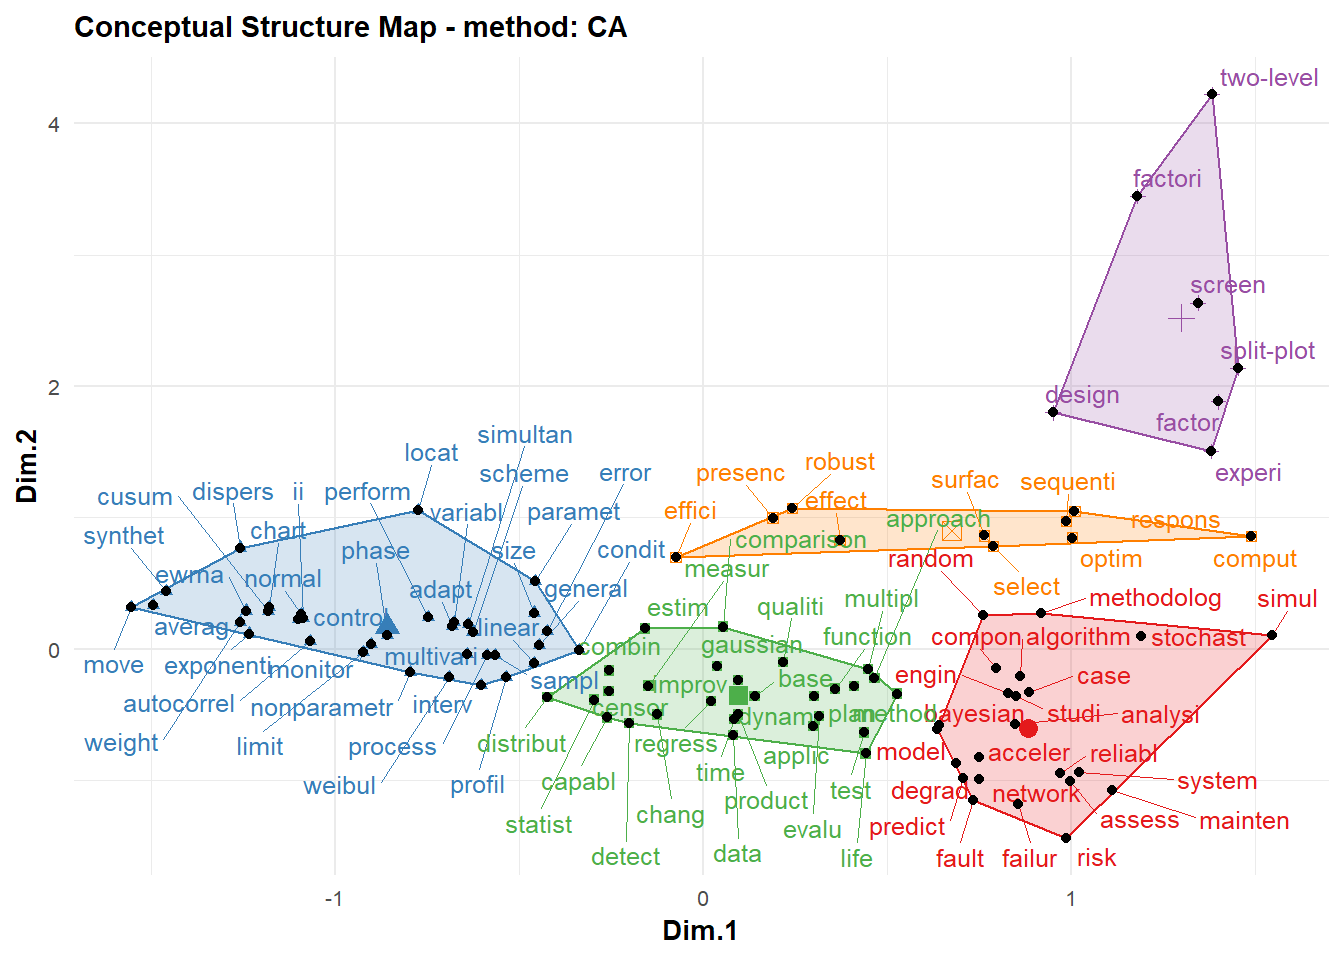
\includegraphics[width=\textwidth, height = 0.6\textheight, keepaspectratio, frame]{Figures/conceptmap-1.png}}
  
  \only<2>{\textbf{(2) In the Frontiers of Statistical Quality Control 12, we had 20 outstanding contributions. The papers considered important application domains such as: web data, multi-stage processes, and single server queues.}
  
  \vspace{\baselineskip}
  
  \textbf{None of the papers explicitly considered monitoring human performance data. However, \textcolor{miamired}{the discussion in Lazariv and Schmid \cite{lazariv2018challenges} can be easily thought of in the context of human performance monitoring applications.}}}
  
  \only<3>{\textbf{(3) If we examine JQT as an example, it had three excellent special issues in 2018:}
  \begin{itemize}
      \item \textbf{``statistical process control on big data streams"}
      \item \textbf{``quality engineering in advanced manufacturing"}
      \item \textbf{``reliability and maintenance modeling with big data"}
  \end{itemize}
  
  \vspace{\baselineskip}
  
  \textbf{None of the 19 special issue papers considered human performance modeling.}
  }
  
  \only<4>{
  \textbf{(4) Note: In ISQC 2019, we have had two excellent talks that discuss the combination of CPS technologies with individualized health monitoring.}
  
  \vspace{\baselineskip}
  
  \begin{itemize}
      \item \textbf{\textcolor{miamired}{``Monitoring Two-state Processes Using Indirectly Observed Data"} by: O. Hryniewicz, K. Kaczmarek-Majer, K. Opara}
      \item \textbf{\textcolor{miamired}{``Personalized Health Management for Elderly Care"} by: KL Tsui}
  \end{itemize}
  
  \vspace{\baselineskip}
  
  \begin{dBox}
    \textbf{So hopefully, these talks lead to increased interests in an important area that affects public interests and health.}
  \end{dBox}
  
  }
  
  \only<5>{
  \begin{dBox}
    \textbf{Why should SQC care about human performance monitoring applications?} \textbf{\textcolor{gray}{If you think of advanced manufacturing, which is our most common application area in SQC and industrial statistics:}}
  \end{dBox}
  
  \vspace{\baselineskip}
  
  \textbf{In addition to the potential of CPS technologies, there is a direct link of human performance to quality outcomes. In a recent review of 73 published empirical studies by \cite{kolus2018production}, the authors clearly stated that:}
  
  \begin{quotation}
      \noindent \textbf{\textcolor{miamired}{Quality deficits were associated with undesirable human effects of workload like fatigue and injury-related risk factors. Forty-six percent of the studies reported on efforts to improve HF in the [operations systems] with effect sizes for quality improvements reaching up to 86\%.}}
  \end{quotation}
  }
  
\end{frame}

\section{How SQC can Inform/Augment AI for CPS Applications}

% Frame 11 - How People think about AI/Machine Learning
\begin{frame}{\textbf{Common Frameworks for AI/ Machine Learning}}
    
    \only<1>{
    \begin{table}[h]
        \centering
        \begin{tabular}{|l|l|l|}
        \hline 
             \textbf{The KDD Process} & \textbf{SEMMA} & \textbf{CRISP-DM} \\ \hline \hline 
             \rowcolor{gray!30}
             Pre KDD & ------------- & Business understanding \\ \hline \hline 
             Selection & Sample & \multirow{2}{*}{Data understanding} \\ \cline{1-2}
             Pre processing & Explore & \\ \hline \hline 
             \rowcolor{gray!30}
             Transformation & Modify & Data preparation \\ \hline \hline 
             Data mining & Model & Modeling \\ \hline \hline 
             \rowcolor{gray!30}
             Interpretation/Evaluation & Assessment & Evaluation \\ \hline \hline  
             Post KDD &  ------------- & Deployment \\ \hline \hline 
        \end{tabular}
        \caption{A comparison of the three most commonly used AI/Machine Learning Frameworks. Table adapted from \cite{azevedo2008kdd}.}
        \label{tab:frameworks}
    \end{table}
    }

    \only<2>{
    \begin{dBox}
        \textbf{These three frameworks encourage iterating, but do not provide sufficient guidance to practitioners/ researchers. \textcolor{miamired}{Guidance:} Typically focuses on the data mining / modeling step.}
    \end{dBox}
    
    \centering 
    
    \vspace{0.5\baselineskip}
    
    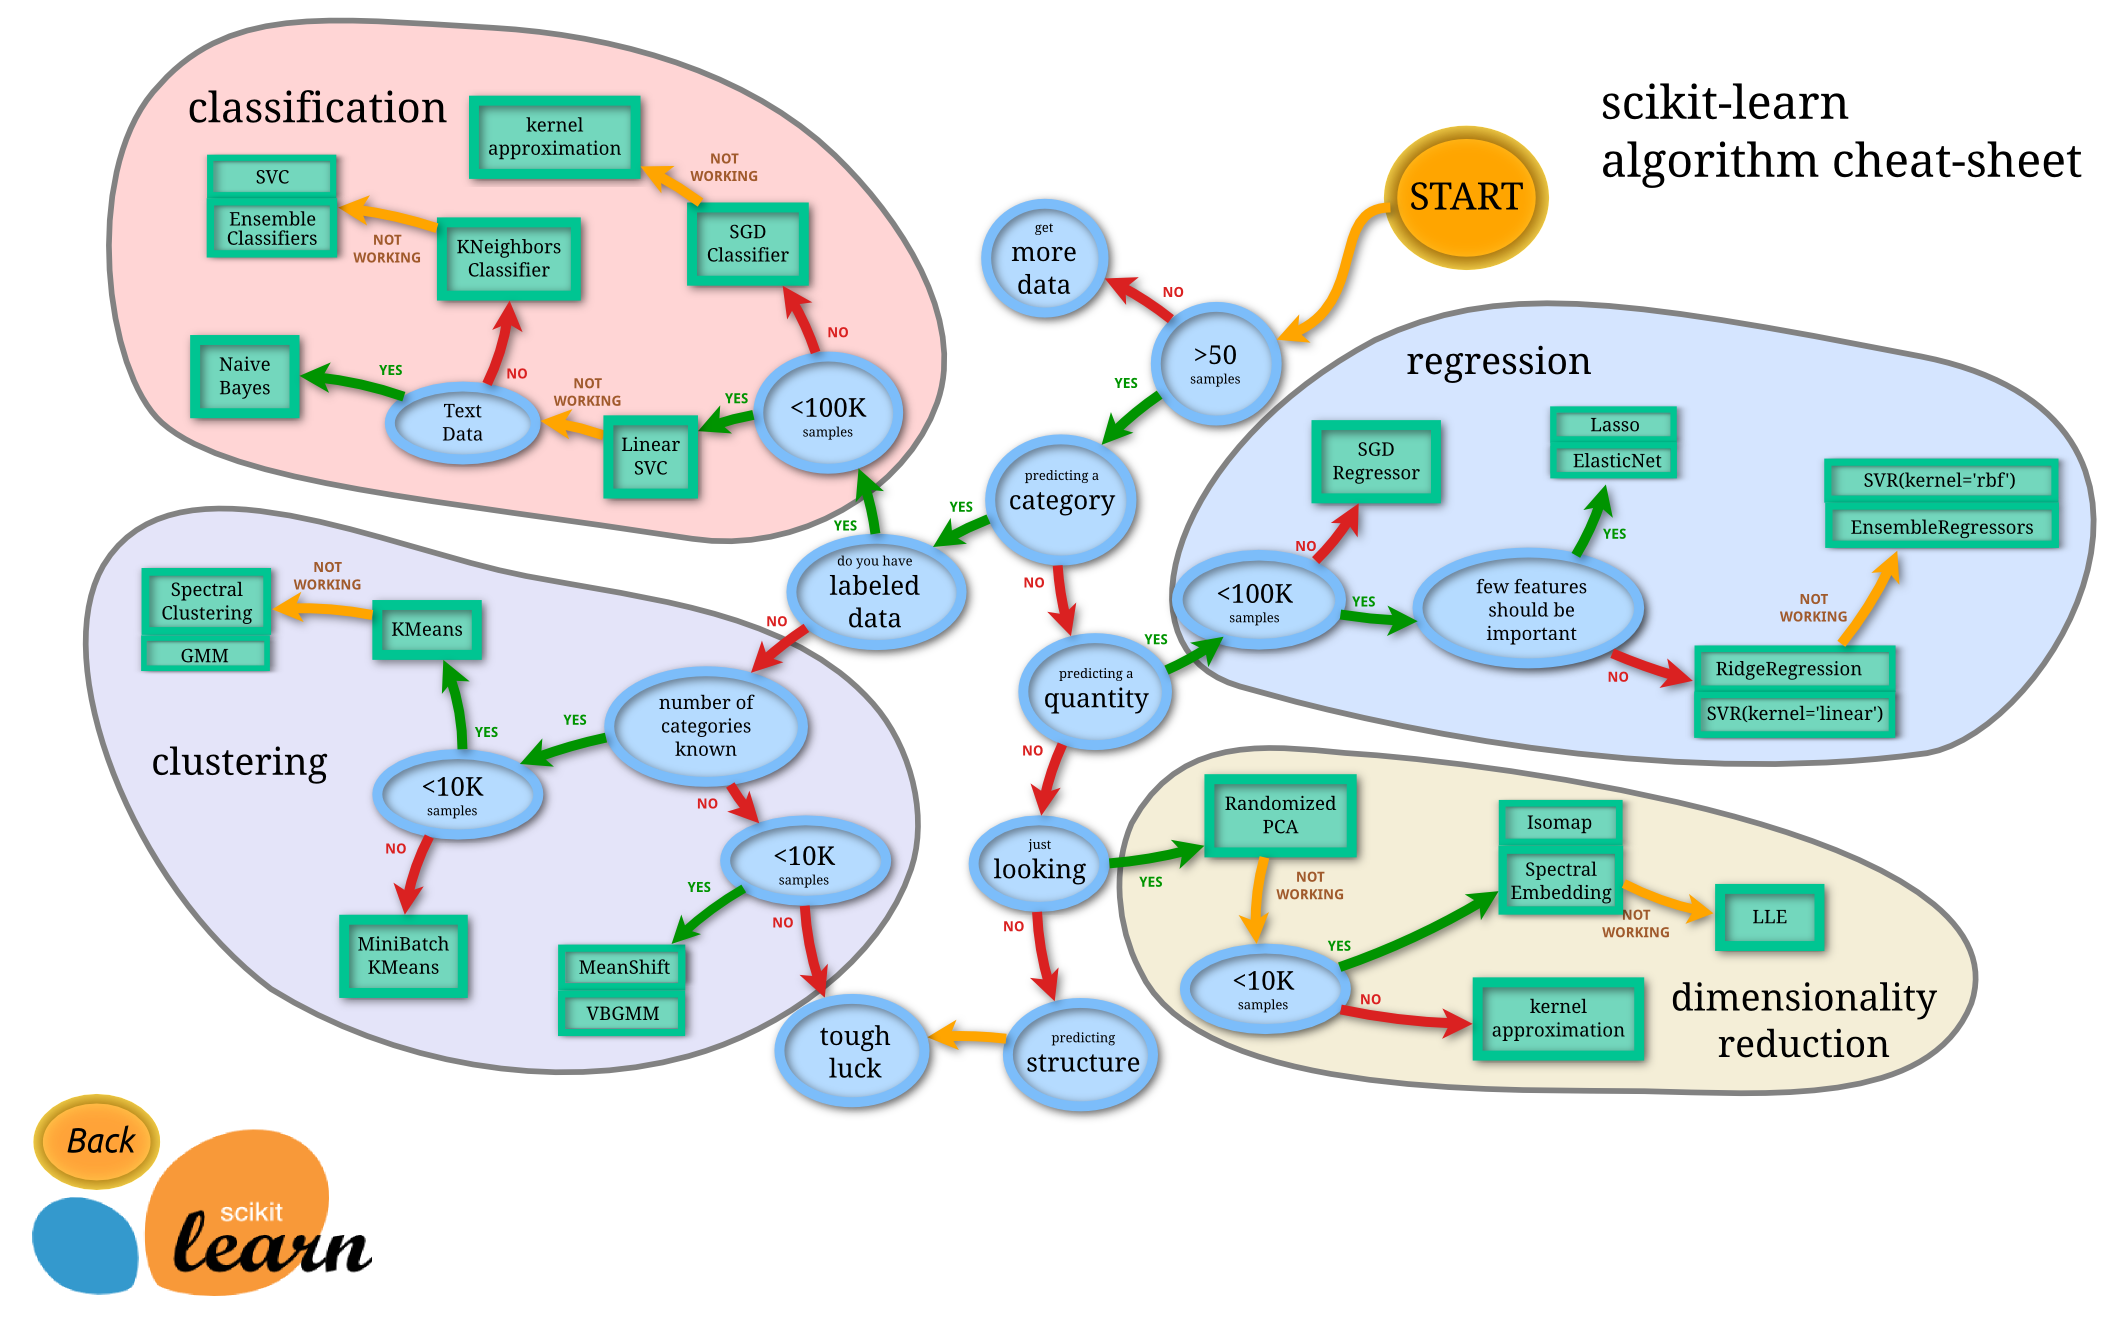
\includegraphics[width=\textwidth, height=0.6\textheight, keepaspectratio, frame]{Figures/ml_map.png} \\
    
    \footnotesize{\textbf{Source:} SciKit-Learn \cite{scikit2019choosing}}
    }
    
\end{frame}

% Frame 12 - Role of SQC Methodologies
\begin{frame}{\textbf{Role of SQC in AI/ ML (CPS) Applications}}
    \begin{figure}[h!]
		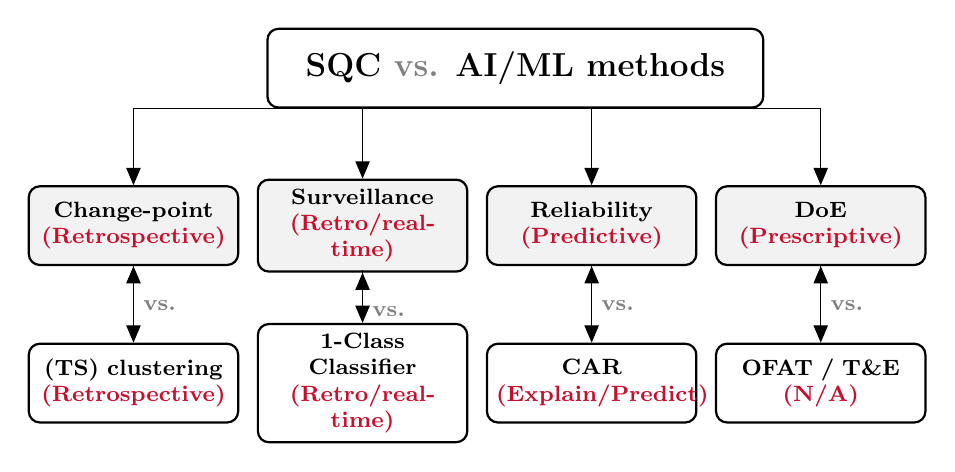
\begin{tikzpicture}[node distance=2cm, font=\footnotesize]
		\tikzstyle{start} = [rectangle, rounded corners, minimum width=0.5\textwidth, minimum height=1cm,text badly centered, text width=0.5\textwidth, draw=black, thick, font=\large]
		
		\tikzstyle{categories} = [rectangle, rounded corners, minimum width=0.2\textwidth, minimum height=1cm,text centered, text width=0.2\textwidth, draw=black, fill=gray!10, thick]
		
		\tikzstyle{ml} = [rectangle, rounded corners, minimum width=0.2\textwidth, minimum height=1cm,text centered, text width=0.2\textwidth, draw=black, thick]
		
		\tikzstyle{arrow} = [->,>= triangle 45]
		\tikzstyle{arrow2} = [<->,>= triangle 45]
		%-------------------------------------------------------
		% Begining of the creation of the figure
		\node (start) [start] {\textbf{\textcolor{black}{SQC \textcolor{gray}{vs.} AI/ML methods}}};
		
			\node (n1) [categories, below of = start, xshift=-0.4\textwidth]{\textbf{\textcolor{black}{Change-point \\
			\textcolor{miamired}{(Retrospective)}}}};
			\node (n2) [categories, right of = n1,xshift=0.075\textwidth]{\textbf{\textcolor{black}{Surveillance \\ \textcolor{miamired}{(Retro/real-time)}}}};
			\node (n3) [categories, right of = n2,xshift=0.075\textwidth]{\textbf{\textcolor{black}{Reliability \\ \textcolor{miamired}{(Predictive)}}}};
			\node (n4) [categories, right of = n3, xshift=0.075\textwidth]{\textbf{\textcolor{black}{DoE \\\textcolor{miamired}{(Prescriptive)}}}};
			
			\node (n5) [ml, below of = n1]{\textbf{\textcolor{black}{(TS) clustering \\
			\textcolor{miamired}{(Retrospective)}}}};
			
			\node (n6) [ml, below of = n2]{\textbf{\textcolor{black}{1-Class Classifier \\
			\textcolor{miamired}{(Retro/real-time)}}}};	
		    
		    \node (n7) [ml, below of = n3]{\textbf{\textcolor{black}{CAR \\
			\textcolor{miamired}{(Explain/Predict)}}}};
		    
		    \node (n8) [ml, below of = n4]{\textbf{\textcolor{black}{OFAT / T\&E \\
			\textcolor{miamired}{(N/A)}}}};
		    
		\draw [arrow] (start.south) -| (n1);
		\draw [arrow] (start.south) -| (n2);
		\draw [arrow] (start.south) -| (n3);
		\draw [arrow] (start.south) -| (n4);
		
		\draw [arrow2] (n1.south) -| node[anchor=west, yshift=-0.5cm]{\textbf{\textcolor{gray}{vs.}}}(n5);
		\draw [arrow2] (n2.south) -| node[anchor=west, yshift=-0.5cm]{\textbf{\textcolor{gray}{vs.}}}(n6);
		\draw [arrow2] (n3.south) -| node[anchor=west, yshift=-0.5cm]{\textbf{\textcolor{gray}{vs.}}}(n7);
		\draw [arrow2] (n4.south) -| node[anchor=west, yshift=-0.5cm]{\textbf{\textcolor{gray}{vs.}}}(n8);
		\end{tikzpicture}

\end{figure}

\pause

\begin{eBox}
    \textbf{Let us examine three examples (wearables, trucking \& cyber security).}
\end{eBox}

\end{frame}

\section{Example Applications}

\subsection{Wearable Sensors for Physical Fatigue Management}

% Frame 14
\begin{frame}{\textbf{Wearables: How I got involved?}}
    
\end{frame}


% Miao's Section
\subsection{Trucking Safety}

% Frame data sources M1
\begin{frame}{\textbf{Data sources}}
    \begin{itemize}
      \item \textbf{Real-time pings}: real-time data on vehicle number, date and time, latitude, longitude, driver identification number (ID), and speed. Collected every 1 to 10 minutes.
      \item \textbf{safety critical events, SCEs}: 1) hard brake (HB), 2) headway (HW), 3) collision mitigation (CM), and 4) rolling stability (RS).
      \item \textbf{Driver demographics}: driver \textit{age}.
      \item \textbf{Road geometry}: \textit{speed limits} and \textit{the number of lanes} from the OpenStreetMap API.
      \item \textbf{Weather}: \textit{precipitation intensity}, \textit{precipitation probability}, \textit{wind speed}, and \textit{visibility}, from the Dark Sky API.
  \end{itemize}
\end{frame}

% Frame data transformation M2
\begin{frame}{\textbf{Data transformation}}
    \begin{itemize}
      \item \textbf{Trips}:  real-time ping stopped for $\geq20$ minutes, the ping data will be separated into two different trips. A trip is \textit{short continuous driving intervals} with a mean length of 1.8 hours.
      \item \textbf{Half-hour intervals}: trip length is heterogeneous (5 minutes to $\geq8$ hours),  so trips were further divided into half-an-hour fixed intervals.
      \item \textbf{Shifts}: the trips will be further divided into different shifts if the driver was not moving for at least eight hours. A shift is therefore a long driving time with \textit{intermittent short rests} (20 minutes to $<8$ hours).
      \item \textbf{A proxy of driver fatigue}: cumulative summation of interval time within a shift for each driver as the \textit{cumulative driving time}.
  \end{itemize}
\end{frame}

% Frame data merging (flow chart) M3
\begin{frame}{\textbf{Data merging}}
\centering
  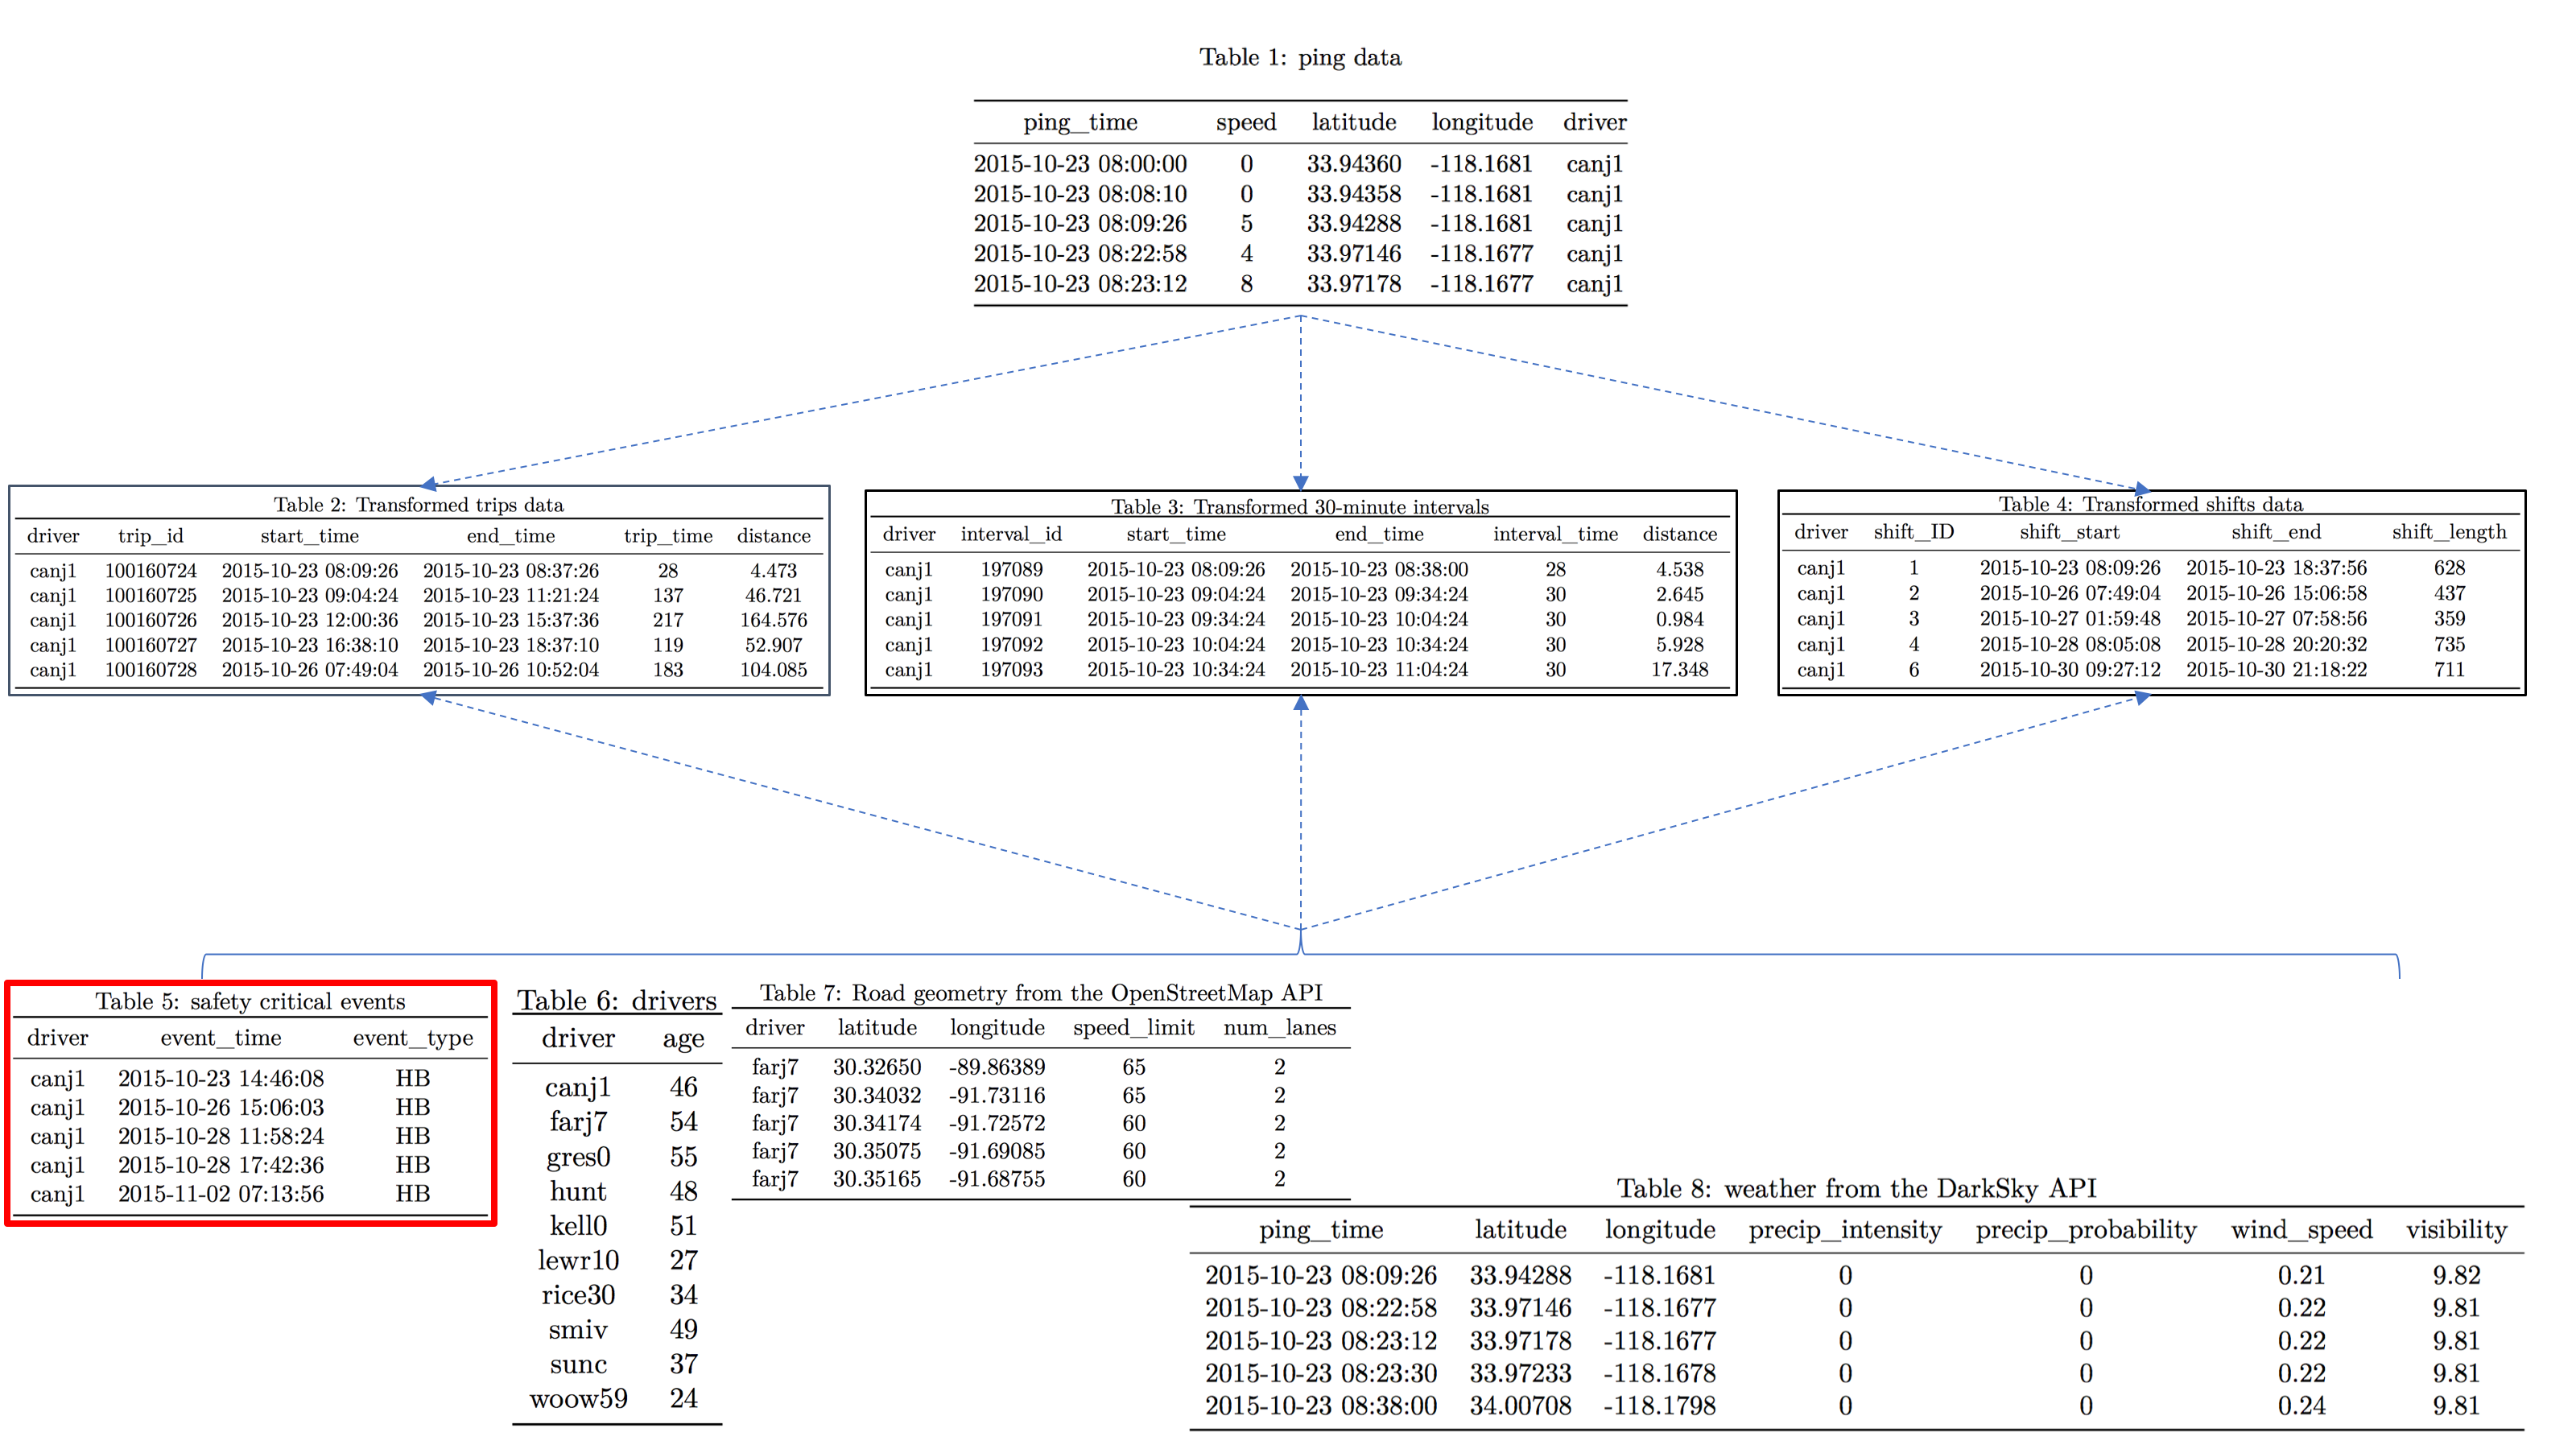
\includegraphics[width=\textwidth, height = \textheight, keepaspectratio, frame]{Figures/flow_chart.png}
\end{frame}

% Frame logit
\begin{frame}{\textbf{Bayesian random-effects logistic regression}}
\begin{equation}\label{eq:logit}
\begin{split}
Y_{i} &\sim \text{Bernoulli}(p_{i})\\
\log\frac{p_{i}}{1-p_{i}} &= \beta_{0, d(i)} + \beta_{1, d(i)} \cdot \text{CT}_i + \sum_{j=1}^{J} x_{ij}\beta_j\\
\beta_{0, d} &\sim \text{i.i.d. } N(\mu_0, \sigma_0^2), \quad d = 1, 2, \cdots, D\\
\beta_{1, d} &\sim \text{i.i.d. } N(\mu_1, \sigma_1^2), \quad d = 1, 2, \cdots, D
\end{split}
\end{equation}
\begin{itemize}
    \item $Y_i$: whether SCEs occurred during the interval, 0 or 1,
    \item CT$_i$: cumulative driving time,
    \item $\beta_{0, d}$: random intercepts for each driver,
    \item $\beta_{1, d}$: random slopes for CT$_i$ for each driver,
    \item $x_{ij}$: covariates, including age, road geometry, and weather.
\end{itemize}
\end{frame}

% Frame Poisson
\begin{frame}{\textbf{Bayesian random-effects Poisson regression}}
\begin{equation}\label{eq:pois}
\begin{split}
Y_{i}  & \sim \text{Poisson}(T_i\cdot\lambda_i)\\
\log\lambda_{i} & =\beta_{0, d(i)} + \beta_{1, d(i)} \cdot \text{CT}_i + \sum_{j=1}^{J} x_{ij}\beta_j\\
\beta_{0, d} &\sim \text{i.i.d. } N(\mu_0, \sigma_0^2), \quad d = 1, 2, \cdots, D\\
\beta_{1, d} &\sim \text{i.i.d. } N(\mu_1, \sigma_1^2), \quad d = 1, 2, \cdots, D
\end{split}
\end{equation}
\begin{itemize}
    \item $Y_i$: the number of SCEs during the interval, a non-negative integer,
    \item $T_i$: length of the interval as an offset term,
    \item CT$_i$: cumulative driving time,
    \item $\beta_{0, d}$: random intercepts for each driver,
    \item $\beta_{1, d}$: random slopes for CT$_i$ for each driver,
    \item $x_{ij}$: covariates, including age, road geometry, and weather.
\end{itemize}
\end{frame}

% Frame priors
\begin{frame}
\textbf{Weakly informative} priors and hyper-priors as recommended by Gelman \cite{gelman2017prior}.
\begin{equation}
	\label{eq:prior}
	\begin{split}
		\mu_0 & \sim N(0, 5^2)\\
		\mu_1 & \sim N(0, 5^2)\\
		\sigma_0 & \sim \text{Gamma}(1, 1)\\
		\sigma_1 & \sim \text{Gamma}(1, 1)\\
		\beta_2, \beta_3, \cdots, \beta_J  & \sim N(0, 10^2)
	\end{split}
\end{equation}
\begin{itemize}
    \item $\mu_0, \sigma_0$: hyper-parameters for $\beta_{0, d}$,
    \item $\mu_1, \sigma_1$: hyper-parameters for $\beta_{1, d}$,
    \item $\beta_2, \beta_3, \cdots, \beta_J$: fixed parameters for covariates $x_{ij}$.
\end{itemize}
\end{frame}

% Frame NHPP - theory
\begin{frame}{\textbf{Non-homogeneous Poisson process: introduction}}
\begin{itemize}
    \item The \textbf{intensity function} of a point process is $$\lambda(t) = \lim_{\Delta t \rightarrow 0}\frac{P(N(t, t+\Delta t] \geq 1)}{\Delta t}$$
    \item \textbf{Nonhomogeneous Poisson Process (NHPP)}: a Poisson process whose intensity function is non-constant.
    \item \textbf{Power law process (PLP)}: the intensity function of a NHPP is $$\lambda(t) = \frac{\beta}{\theta}\bigg(\frac{t}{\theta}\bigg)^{\beta-1}, \quad \beta > 0, \theta > 0.$$
    \item $\beta$ is the shape parameter.  $\theta$ is the scale parameter.
    \item $\beta > 1 \rightarrow$ reliability deterioration; $\beta > 1 \rightarrow$ reliability improvement.
\end{itemize}
\end{frame}

% Frame NHPP - notations
\begin{frame}{\textbf{Non-homogeneous Poisson process: data}}
\begin{columns}
\begin{column}{.64\textwidth}
\begin{itemize}
\item $T_{d, s, i}$: the time to the $d$-th driver's $s$-th shift's $i$-th critical event,
\item $d$: driver index, $d = 1, 2, \cdots, D$
\item $s$: shift index, $s = 1, 2, \cdots, S_d$,
\item $i$: SCE index, $i = 1, 2, \cdots, n_{d, S_d}$
\item $n_{d,s}$: the total number critical events of $d$-th driver's $s$-th shift. 
\end{itemize}
\end{column}
\hfill
\begin{column}{.35\textwidth}
\begin{figure}
  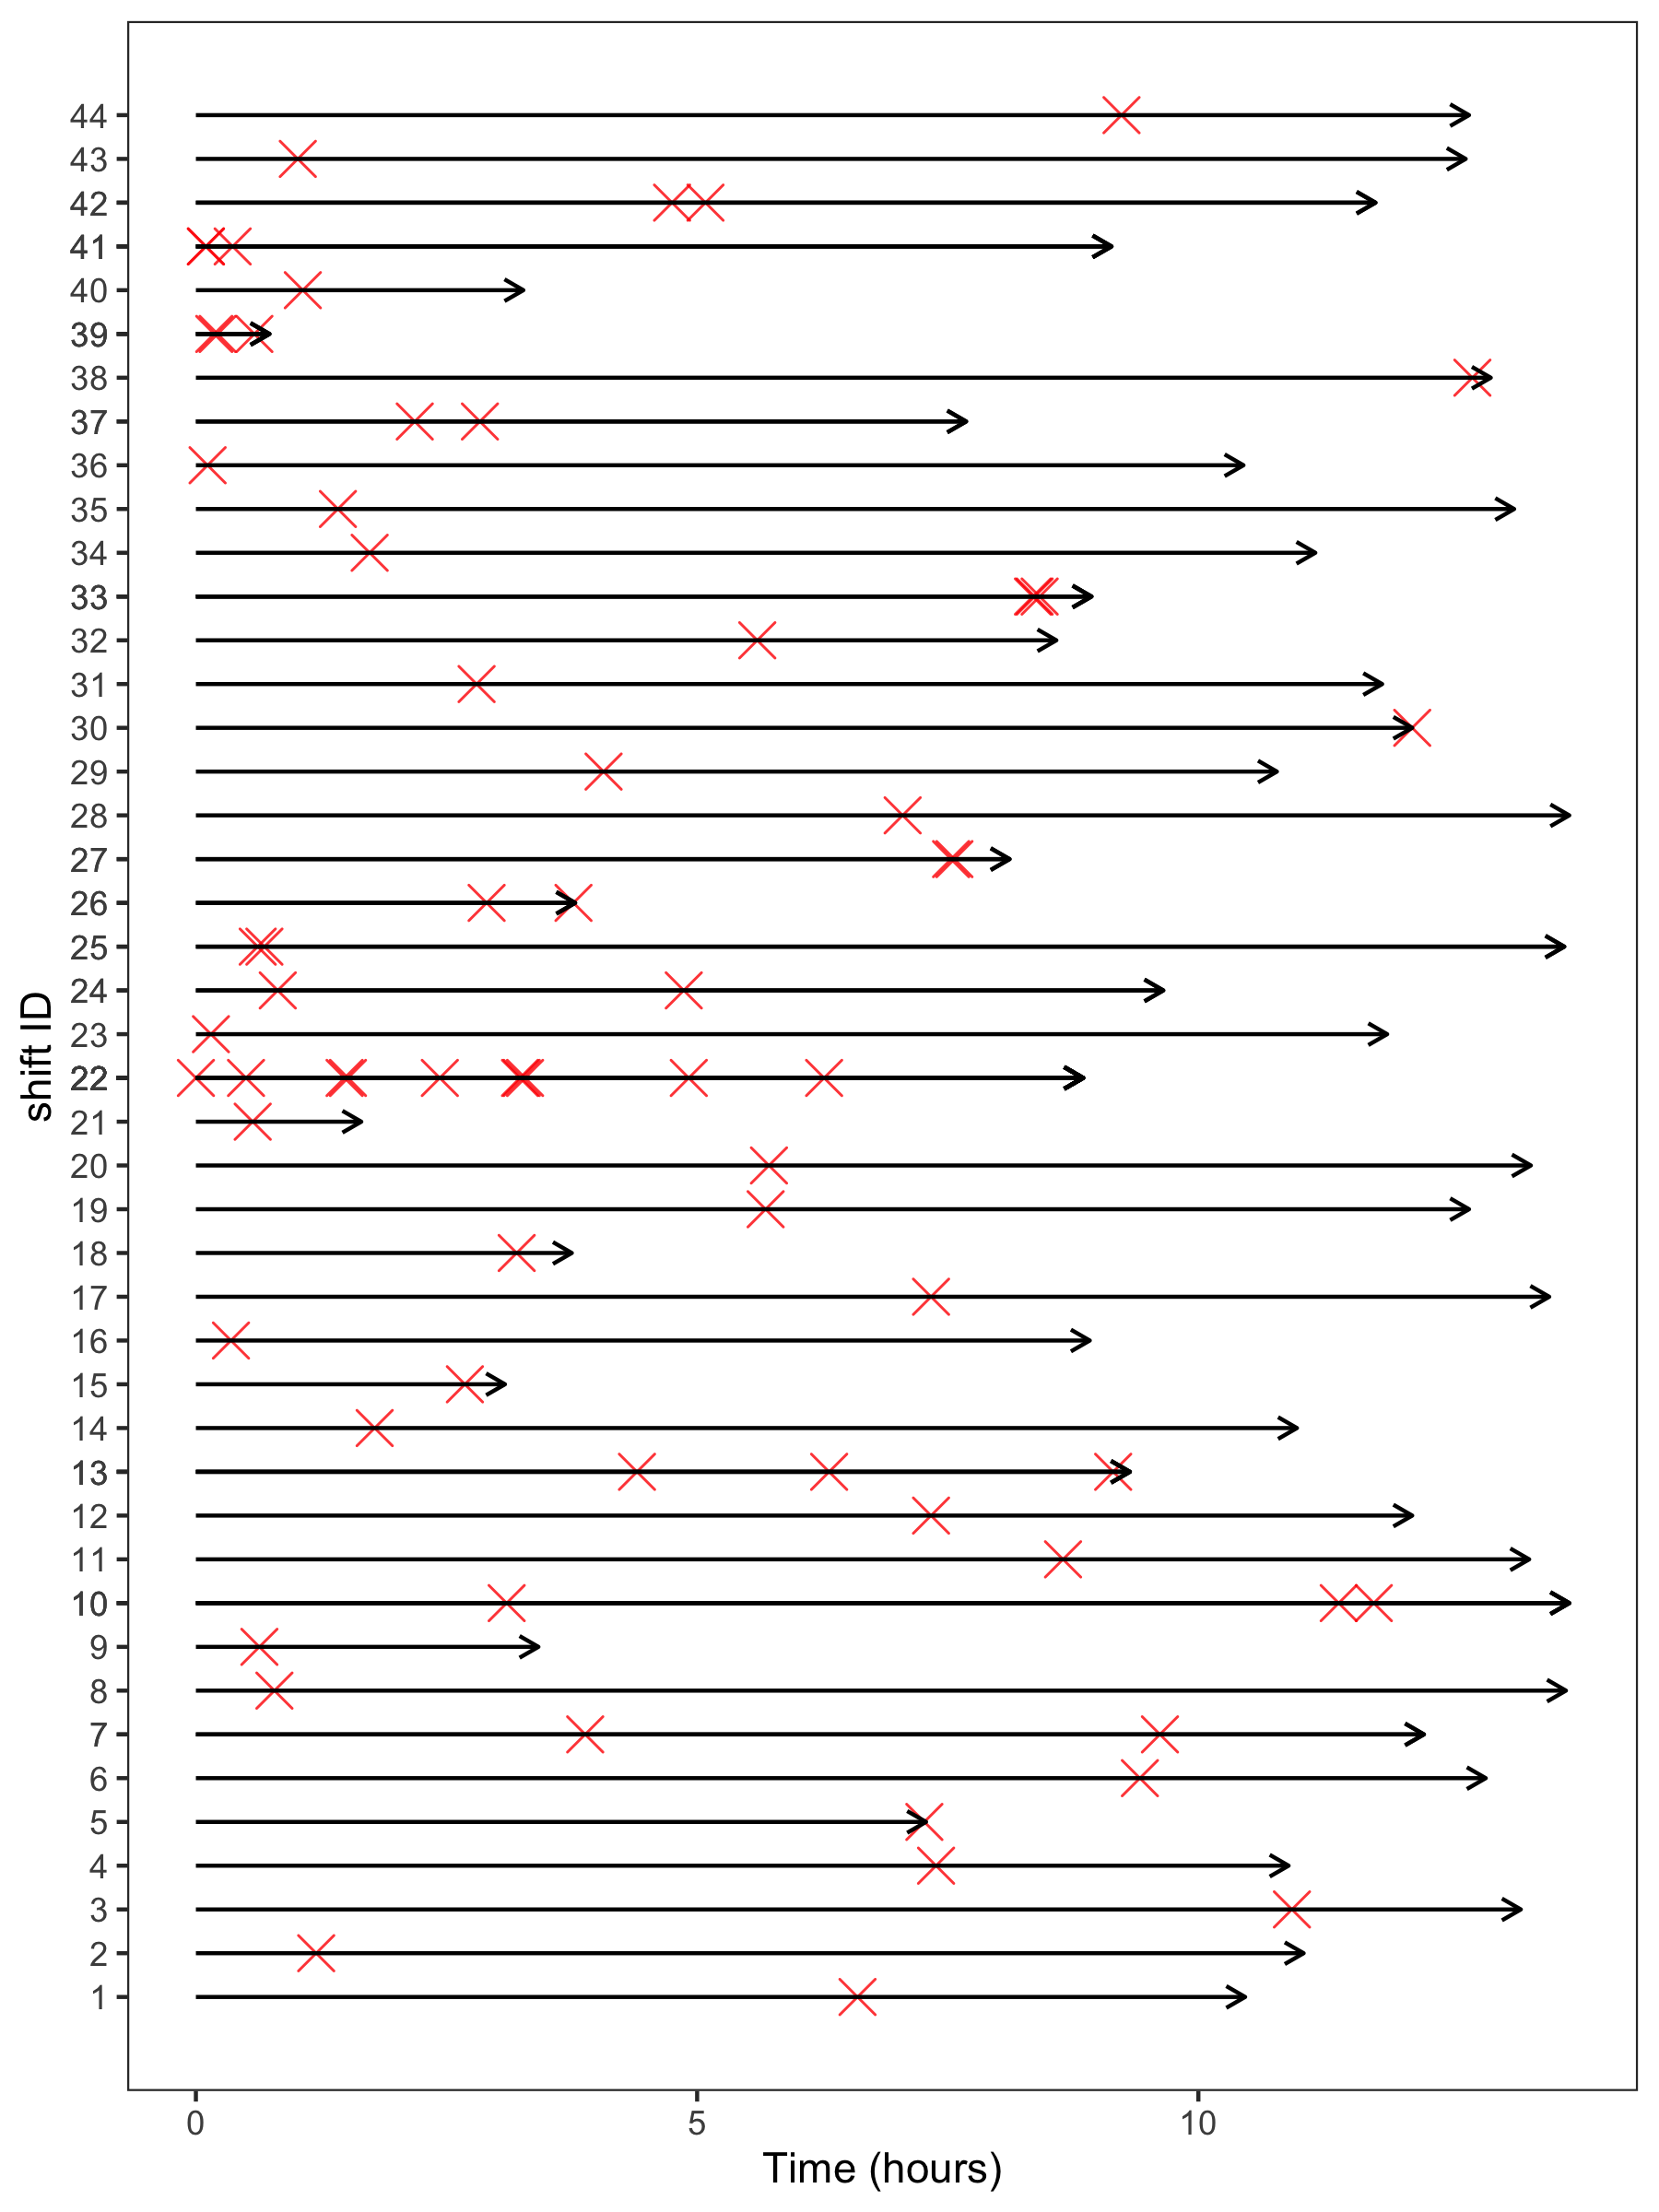
\includegraphics[width=\textwidth]{Figures/t2events_arrow_plot.png}
  \caption{Arrow plot of time to SCEs in each shift}
\end{figure}
\end{column}
\end{columns}
\end{frame}

% Frame NHPP - stats model
\begin{frame}{\textbf{Bayesian random-intercepts NHPP}}
\begin{equation}\label{eq:nhpp}
\begin{aligned}
T_{d, s, 1}, T_{d, s, 2}, \cdots , T_{d, s, n_{d, s}} & \sim \text{PLP}(\beta, \theta_{d, s})\\
\beta & \sim \text{Gamma}(1, 1)\\
\log\theta_{d, s} &= \gamma_{0d} + \gamma_{1}x_{d, s, 1} + \gamma_{2}x_{d, s, 2} + \cdots + \gamma_{k}x_{d, s, k}\\
\gamma_{01}, \gamma_{02}, \cdots, \gamma_{0D} & \sim \text{i.i.d. }N(\mu_0, \sigma_0^2)\\
\gamma_1, \gamma_2, \cdots, \gamma_k & \sim \text{i.i.d. }N(0, 10^2)\\
\mu_0 &\sim N(0, 5^2) \\
\sigma_0 &\sim \text{Gamma}(1, 1)
\end{aligned}
\end{equation}
\begin{itemize}
    \item a fixed $\beta$ across drivers, 
    \item random parameters $\theta_{d, s}$ across drivers
    \item $\theta_{d, s}$: random intercepts $\gamma_{0d}$ for scale parameter $\theta$,
    \item $x_{d, s, k}$: covariates.
\end{itemize}
\end{frame}

% Frame - Bayesian estimation
\begin{frame}{\textbf{Bayesian estimation with rstan}}
\begin{columns}
\begin{column}{.65\textwidth}
\begin{itemize}
    \item Hamiltonian Monte Carlo with No-U-Turn sampler \cite{hoffman2014no, carpenter2017stan},
    \item 4 chains, 1,000 warm-ups, 2000 iterations,
    \item Convergence diagnostics:
    \begin{itemize}
        \item Gelman-Rubin statistics $\hat{R} < 1.1$ \cite{gelman1992inference},
        \item Effective sample size (ESS) $> 500$,
        \item No divergent transitions after warmup,
        \item Traceplots.
    \end{itemize}
    \item All data and code available at \href{https://github.com/caimiao0714/ISQC2019_truck}{https://github.com/caimiao0714/ISQC2019_truck}.
\end{itemize}
\end{column}
\hfill
\begin{column}{.35\textwidth}
\begin{figure}
  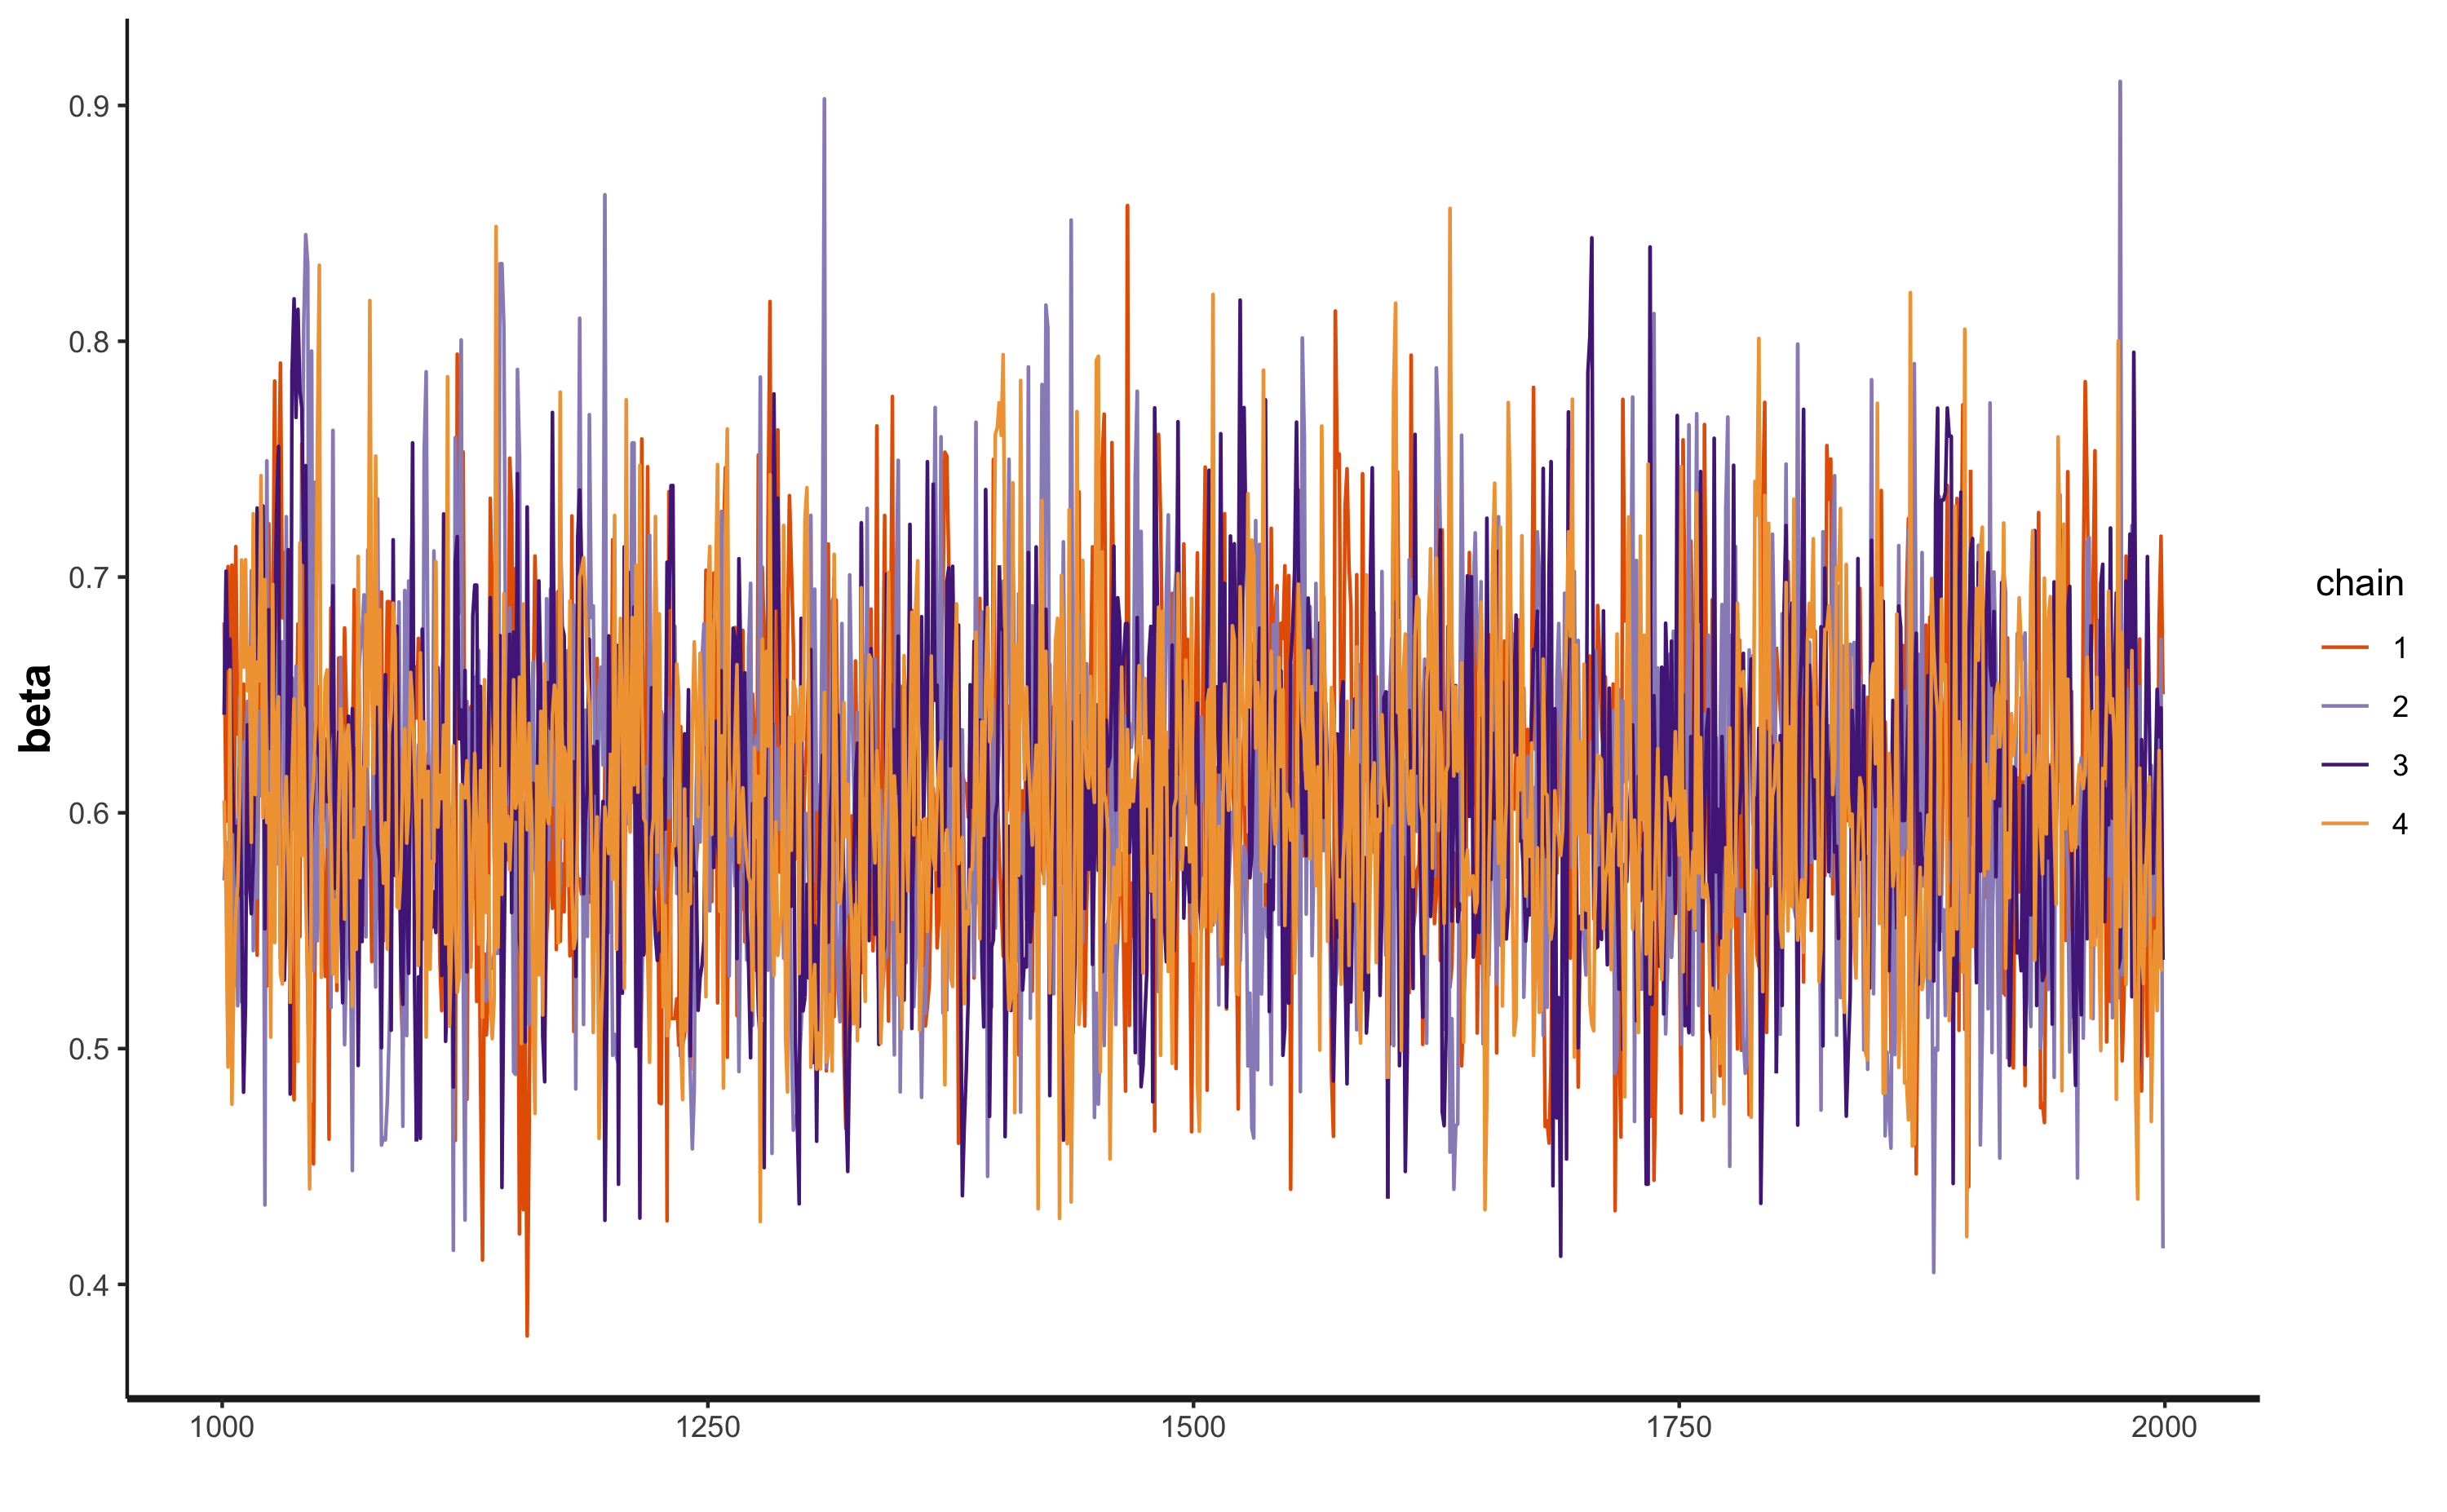
\includegraphics[width=\textwidth]{Figures/traceplot_beta.png}
  \caption{Example trace plot for the shape parameter in NHPP}
\end{figure}
\end{column}
\end{columns}
\end{frame}

% Frame - results: logit and Poisson
\begin{frame}{\textbf{Results for hierarchical Bayesian logit and Poisson regressions}}
\begin{columns}
\begin{column}{.45\textwidth}
\begin{figure}
  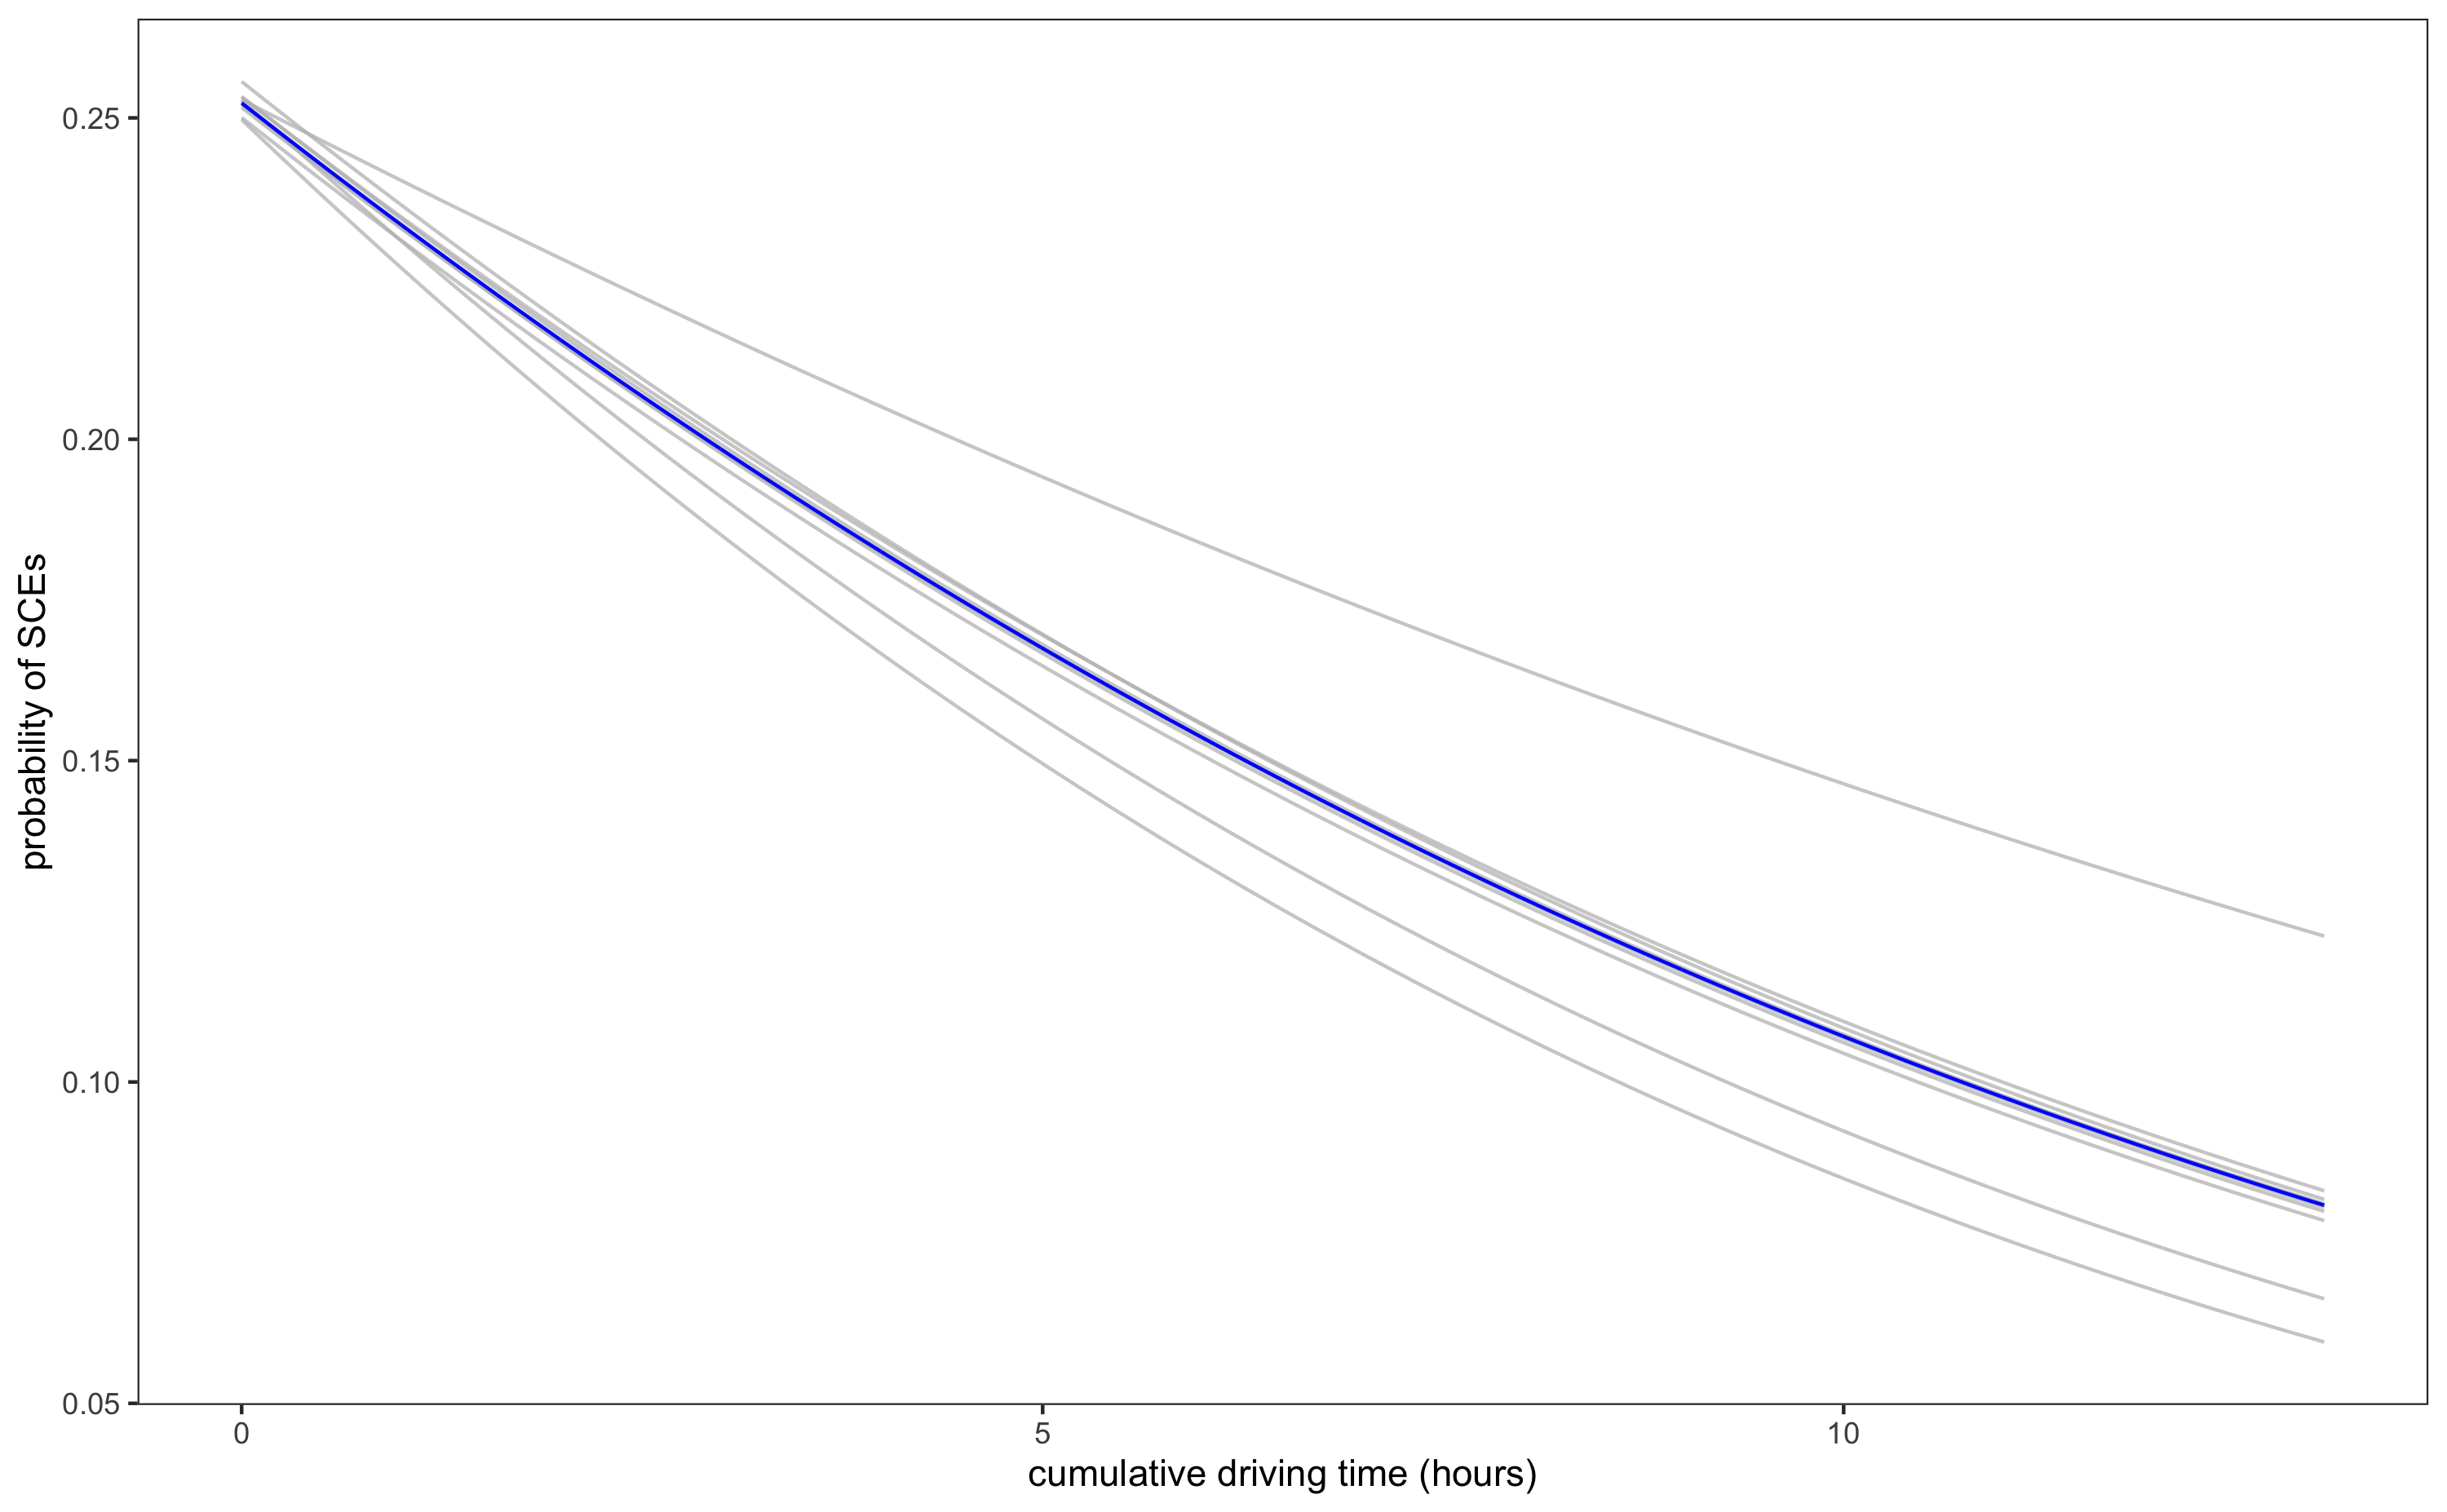
\includegraphics[width=\textwidth]{Figures/fit_logit.png}
  \caption{Cumulative driving time and estimated probability of SCEs from the hierarchical logistic model}
\end{figure}
\end{column}
\hfill
\begin{column}{.45\textwidth}
\begin{figure}
  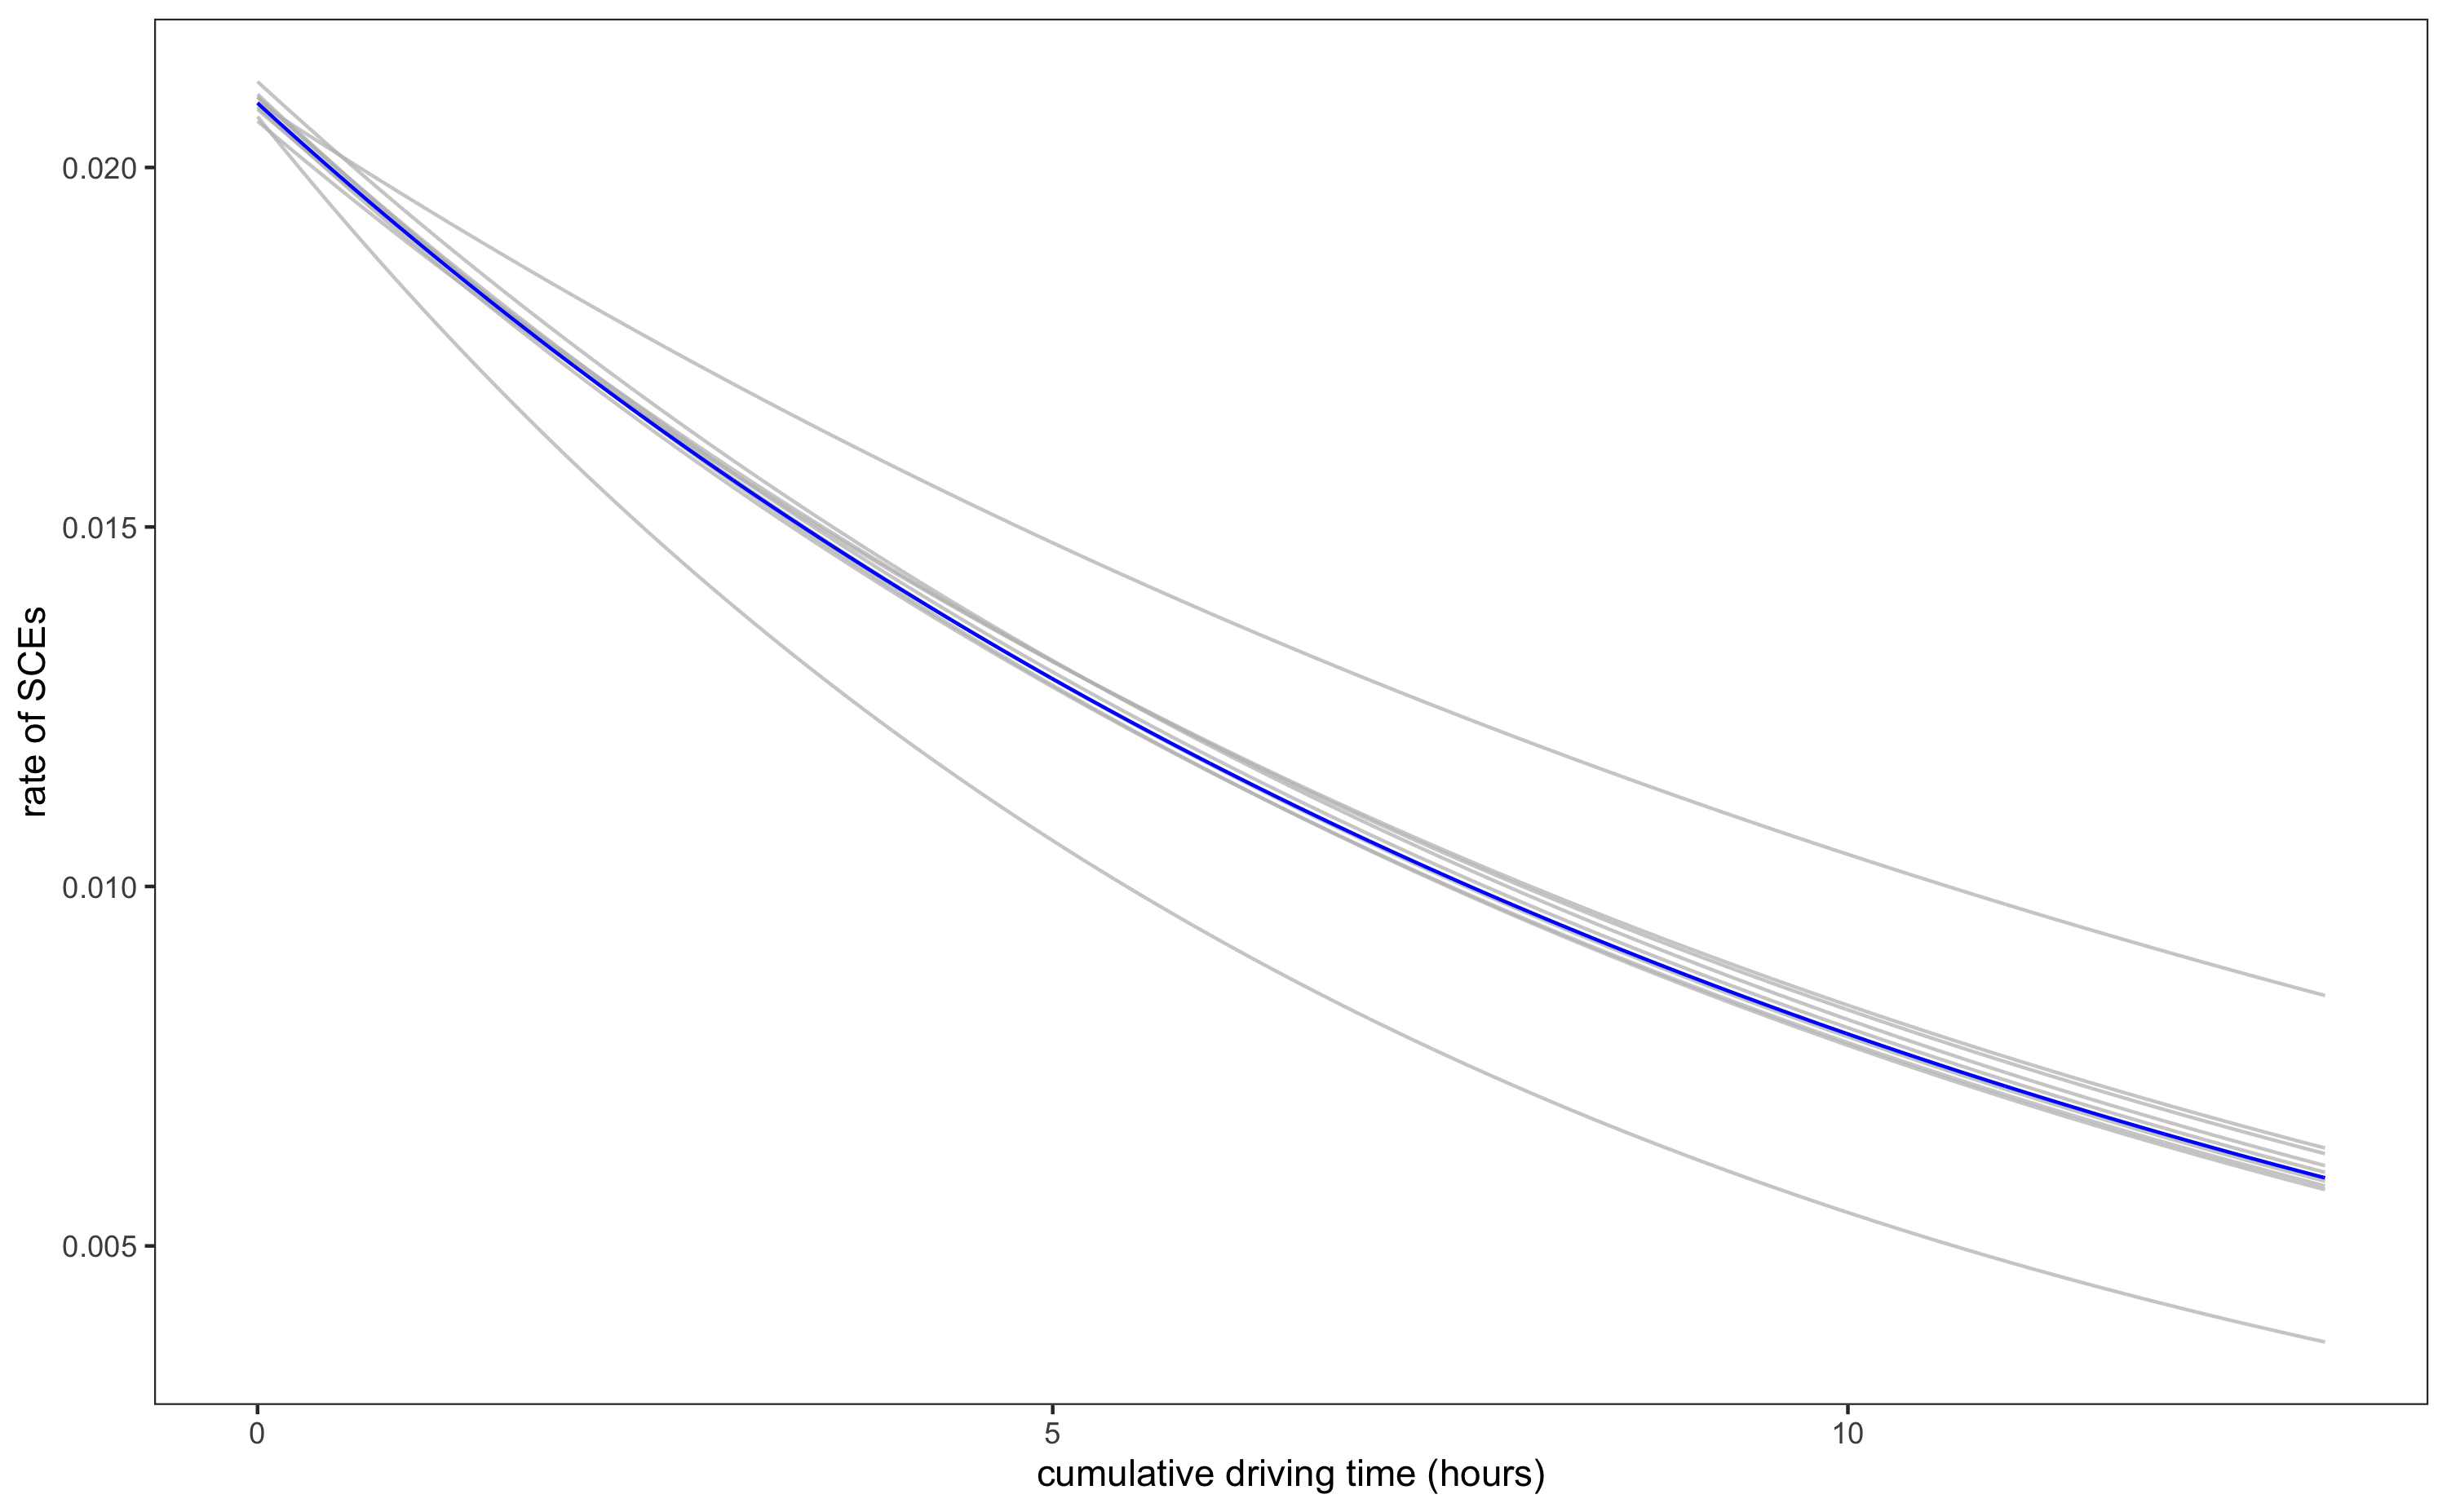
\includegraphics[width=\textwidth]{Figures/fit_Poisson.png}
  \caption{Cumulative driving time and estimated rate of SCEs from the hierarchical Poisson model}
\end{figure}
\end{column}
\end{columns}
\end{frame}

% Frame - results: NHPP
\begin{frame}{Results for hierarchical Bayesian NHPP}
\begin{figure}
  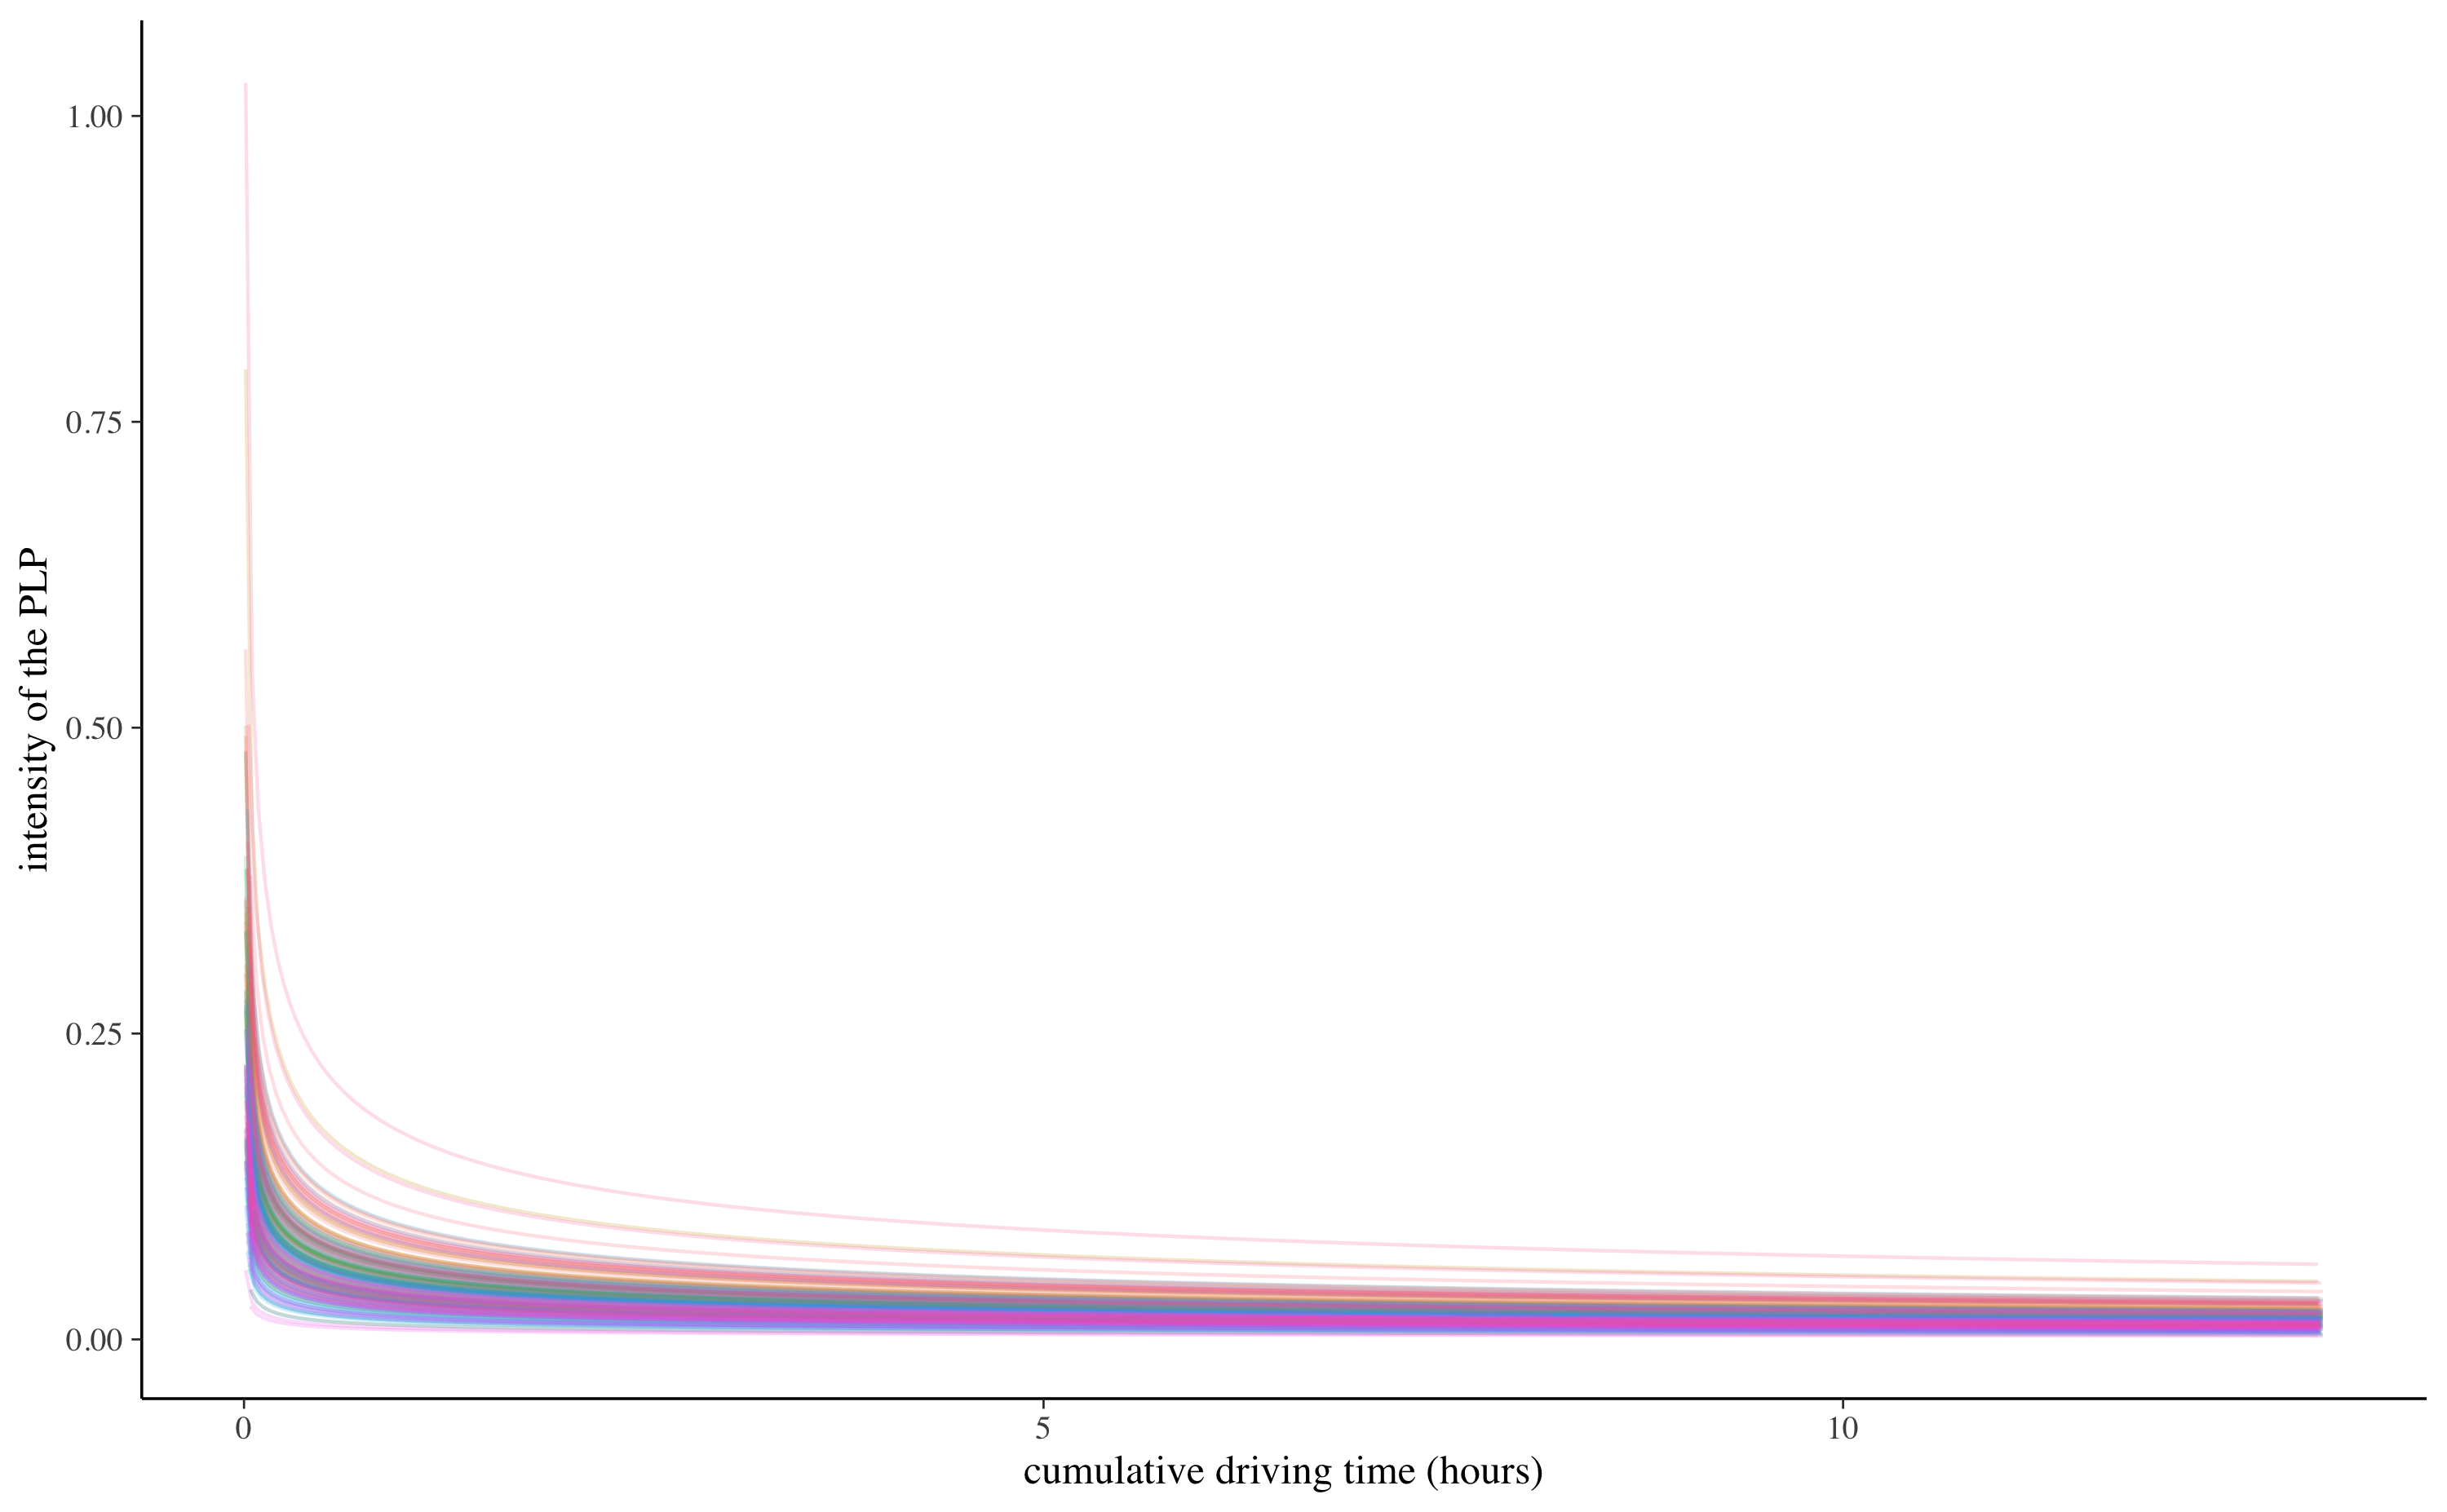
\includegraphics[height=0.45\textheight]{Figures/fit_plp.png}
  \caption{Cumulative driving time and estimated intensity of SCEs from the hierarchical NHPP.}
\end{figure}
\begin{itemize}
    \item 196 shifts for the 10 sample drivers,
    \item y-axis is the intensity of SCEs,
    \item Each line represents a shift, each color represents a driver.
\end{itemize}
\end{frame}

\begin{frame}{Human-Human Authentication}

\begin{itemize}
\item User authentication 
\begin{itemize}
\item Differentiate one human user from another
\end{itemize}
\item Prominent authentication approaches
\begin{itemize}
\item Passwords
\item Traditional biometrics
\end{itemize}
\end{itemize}
\end{frame}



\begin{frame}{Limitations of Existing User Authentication Solutions}

\begin{itemize}
\item Passwords 
\begin{itemize}
\item Either insecure or unusable 
\end{itemize}
\item Traditional biometrics (e.g., fingerprints)
\begin{itemize}
\item Invasive
\item High rejection rates
\item Require additional hardware
\item Susceptible to impersonation or spoofing 
\end{itemize}
\end{itemize}

\begin{overlayarea}{\textwidth}{0.45\textheight}
\only<2>{
\begin{center}

\includegraphics[width=0.3\linewidth]{Figures/password_usability}
\end{center}
}

\only<3>{
\begin{center}
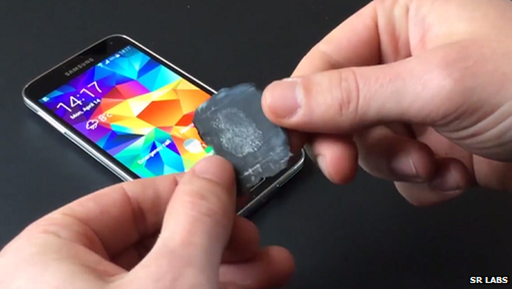
\includegraphics[width=0.3\linewidth]{Figures/spoofing}
\end{center}
}
\end{overlayarea}

\end{frame}



\begin{frame}{Behavioral biometrics}




\begin{itemize}
\item Keystroke dynamics \hfill {\footnotesize{[Monrose et al. ; CCS'97]}}
\item Mouse movement patterns \hfill {\footnotesize{[Zheng et al.; CCS'11]}}
\item Touch gesture biometrics
\begin{itemize}
\item Sliding horizontally and vertically \hfill {\footnotesize{[Frank et al. ; TIFS'13]}}
\item Sliding up, down, left,  and right and tap \hfill {\footnotesize{[Li et al.; NDSS'13]}}
\item Horizontal slide and the pattern unlock  \hfill {\footnotesize{[Luca et al.; CHI'12]}}
\end{itemize}
\end{itemize}


\begin{center}
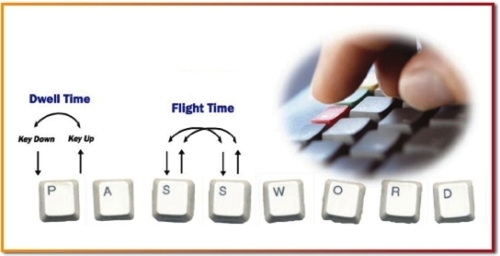
\includegraphics[width=0.3\linewidth]{Figures/bio2}
\end{center}
\end{frame}




\begin{frame}{Gametrics}


\begin{itemize}

\item Interactive game-based behavioral biometrics

\item Why games?

\begin{itemize}
	\item Fully supported by web browsers and touch screen devices
	\item Randomized, interactive and cognitive nature
	\item Sufficient cues can be extracted in a short period of time 
	
\end{itemize}

\end{itemize}

\end{frame}







\begin{frame}{Game Cognitive Task}

\begin{center}
%	\includemedia[
%	activate=pageopen,
%	width=258pt,height=156pt,
%	]{}{Figures/game.swf}
	
	\includemedia[width=0.6\linewidth,height=0.6\linewidth,activate=pageopen,
	passcontext,
	transparent,
	addresource=game.mp4,
	flashvars={source=game.mp4}
	]{
\includegraphics[width=0.6\linewidth]{Figures/game.mp4}}{VPlayer.swf}
	
\end{center}


\end{frame}


\begin{frame}{Features \& Classification Metrics}
\begin{itemize}
\item Features
\begin{itemize}
\item Mouse dynamics / touch gesture  
\item Cognitive ability
\item Others (i.e., distance-based features)
\end{itemize}

\item Classifier
\begin{itemize}
\item Random forest
\end{itemize}

\item Classification metrics 
\begin{itemize}
\item \textbf{False Positive Rate: } Measures the security 
\item \textbf{False Negative Rate:} Measures the usability

\end{itemize}
\end{itemize}

\end{frame}



\begin{frame}{Inter- \& Intra- Session Analysis}
\begin{itemize}
\item Web-based study (MTurk)
\item Data collection methodology:
\begin{itemize}
\item Day 1: 98 participants -- 60 challenges
\item Day 2: 62 participants -- 36 challenges
\item Day 3: 29 participants -- 36 challenges
\end{itemize}

\item Number of successfully completed challenges = 9076
\item Average solving time = 7.5s
\end{itemize}

\end{frame}


\begin{frame}{Inter- \& Intra-Session Results}
%\only<1>{
%\begin{center}
%\includegraphics[width=0.9\linewidth]{Figures/bio-online}
%\end{center}
%}
%
%\only<2>{
%Best results acquired by merging 2 instances and use user specific model
\begin{center}
%\includegraphics[width=0.9\linewidth]{Figures/bio-online-best}
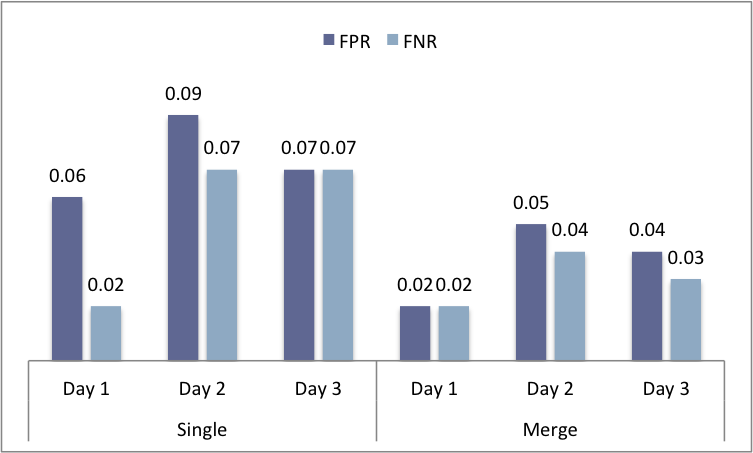
\includegraphics[width=0.9\linewidth]{Figures/result1}
\end{center}
%}

\end{frame}





\begin{frame}{Interactive Biometrics Discussion}

\begin{itemize}
\item Efficiency
\begin{itemize}
\item Short enrollment time
\item Short time to identify the user
\item Building and updating the classifier and testing a new instance take short time
\end{itemize}

\item{Application Scenarios}
\begin{itemize}
\item Point-of-entry
\item Integrated with graphical passwords
\item Fall-back authentication
\end{itemize}

\end{itemize}

\end{frame}


\begin{frame}{Interactive Biometrics Limitations and Future Work}

\begin{itemize}
\item Study the effect of user's behavior variation on the accuracy

\item Test the accuracy when switching devices or hardware

\item  Add more complexity to the game challenges to increase the level of interaction, and improve the overall usability and security

\end{itemize}

\end{frame}

\section*{Bibliography}
% Frame
\begin{frame}[allowframebreaks]{References}%in case more than 1 slide needed
\tiny{
	\bibliographystyle{unsrt}
	\bibliography{refs}
	}
\end{frame}

\maketitle
\end{document}